\documentclass[pdftex,12pt,a4paper]{report}

%------------------------------------------------
%	PACKAGES
%------------------------------------------------

\usepackage{webis}

\usepackage{ucs}

\usepackage[utf8x]{inputenc}

\usepackage{ngerman}

\usepackage[]{algpseudocode}

\usepackage{algorithm}

%------------------------------------------------
%	CONFIGURATION FOR COVER PAGE
%------------------------------------------------

\global\arbeit{Bachelorarbeit}

\global\titel{Mehrbenutzer Multi-Touch-Interaktion mit einem immersiven 3D Bildschirmtisch}

\global\subtitel{}

\global\bearbeiter{Sebastian Stickert}

\global\betreuer{Alexander Kulik, André Kunert}

\global\aufgabensteller{Prof. Dr. Bernd Fröhlich}

\global\abgabetermin{\today} % TODO insert abgabetermin

\global\ort{Weimar} % TODO insert abgabeort

\global\matrikelnummer{110882}

\global\geburtsdatum{21.04.1992}

\global\geburtsort{Rostock}

%------------------------------------------------
%	START DOCUMENT
%------------------------------------------------

\begin{document}


%------------------------------------------------
%	COVER PAGE
%------------------------------------------------

\deckblatt


%------------------------------------------------
%	DECLARATION FOR EXAMINATION OFFICE
%------------------------------------------------

\erklaerung


%------------------------------------------------
%	ABSTRACT
%------------------------------------------------

\begin{abstract}

Dieses Dokument dient als Muster für die Ausarbeitung einer Diplomarbeit
am Lehrstuhl für Webtechnologie und Informationssysteme. 
1 - 2 - 3 Ümläuttest.

\end{abstract}


%------------------------------------------------
%	TABLE OF CONTENTS
%------------------------------------------------

\tableofcontents


%------------------------------------------------
%	THESIS CHAPTERS
%------------------------------------------------

\chapter{Einführung}
\label{chp:einfuehrung}
Hier wird das Kapitel Einführung beschrieben. Das Kapitel besteht aus den Abschnitten \ref{sec:mehrbenutzer_vr_systeme}, \ref{sec:multi_touch_interaktion_mit_3d_szenen} und \ref{sec:ziel_der_arbeit}.

\section{Mehrbenutzer VR-Systeme}
\label{sec:mehrbenutzer_vr_systeme}

Hier steht Inhalt zu Mehrbenutzer VR-Systemen.


\section{Multi-Touch Interaktion mit dreidimensionalen Szenen}
\label{sec:multi_touch_interaktion_mit_3d_szenen}

Hier steht Inhalt zu Multi-Touch Interation mit dreidimensionalen Szenen.


\section{Ziel der Arbeit}
\label{sec:ziel_der_arbeit}

Hier steht Inhalt zum Ziel der Arbeit.

%------------------------------------------------

\chapter{Finger und Hand Tracking auf Grundlage von Maximally Stable Extremal Regions}
\label{chp:mser}
Im Rahmen dieser Arbeit wird ein Bildschirmtisch zur Projektion dreidimensionaler Inhalte verwendet, welcher Multi-Touch Eingaben erlaubt. Gegenüber handgehaltenen Geräten, wie Smartphones, oder Tablets, bietet dieser eine weit größere Interaktionsfläche. Diese begünstigt, wie in Abschnitt \ref{sec:mehrbenutzer_vr_systeme} beschrieben, die kollaborative Arbeit in einem Mehrbenutzerszenario. Die meisten multi-touch gesteuerten Eingabegeräte ordnen alle erkannten Fingerpositionen und deren Bewegung derselben Geste zu. Bei gleichzeitiger Bedienung durch mehrere Nutzer, können nach diesem Ansatz leicht Eingabekonflikte entstehen. Um dem Problem entgegenzuwirken ist ein System erforderlich, welches Aussagen über die hierarchische Zuordnung der Eingabepositionen treffen kann.
\\\\
Hierzu wird in dieser Arbeit die von Ewerling et al. entwickelte Finger und Hand Tracking Implementierung, auf Grundlage des Maximally Stable Extremal Regions (MSER) Algorithmus verwendet \cite{matas:2004, ewerling:2012}. Der theoretische Ansatz dieser Lösung wird in Abschnitt \ref{sec:maximally_stable_extremal_regions} vorgestellt. Abschnitt \ref{sec:technische_voraussetzungen} definiert die technischen Voraussetzungen zur Umsetzung des Multi-Touch Tisches, gefolgt von einem Überblick über die softwareseitige Integration des  MSER Trackings in das genutzte Applikationsframework in Abschnitt \ref{sec:implementierung_mser}. Zuletzt werden die Vorteile und Limitierungen des Systems in Abschnitt \ref{sec:diskussion_mser} diskutiert.


\section{Maximally Stable Extremal Regions}
\label{sec:maximally_stable_extremal_regions}

\begin{figure}
	\begin{center}
		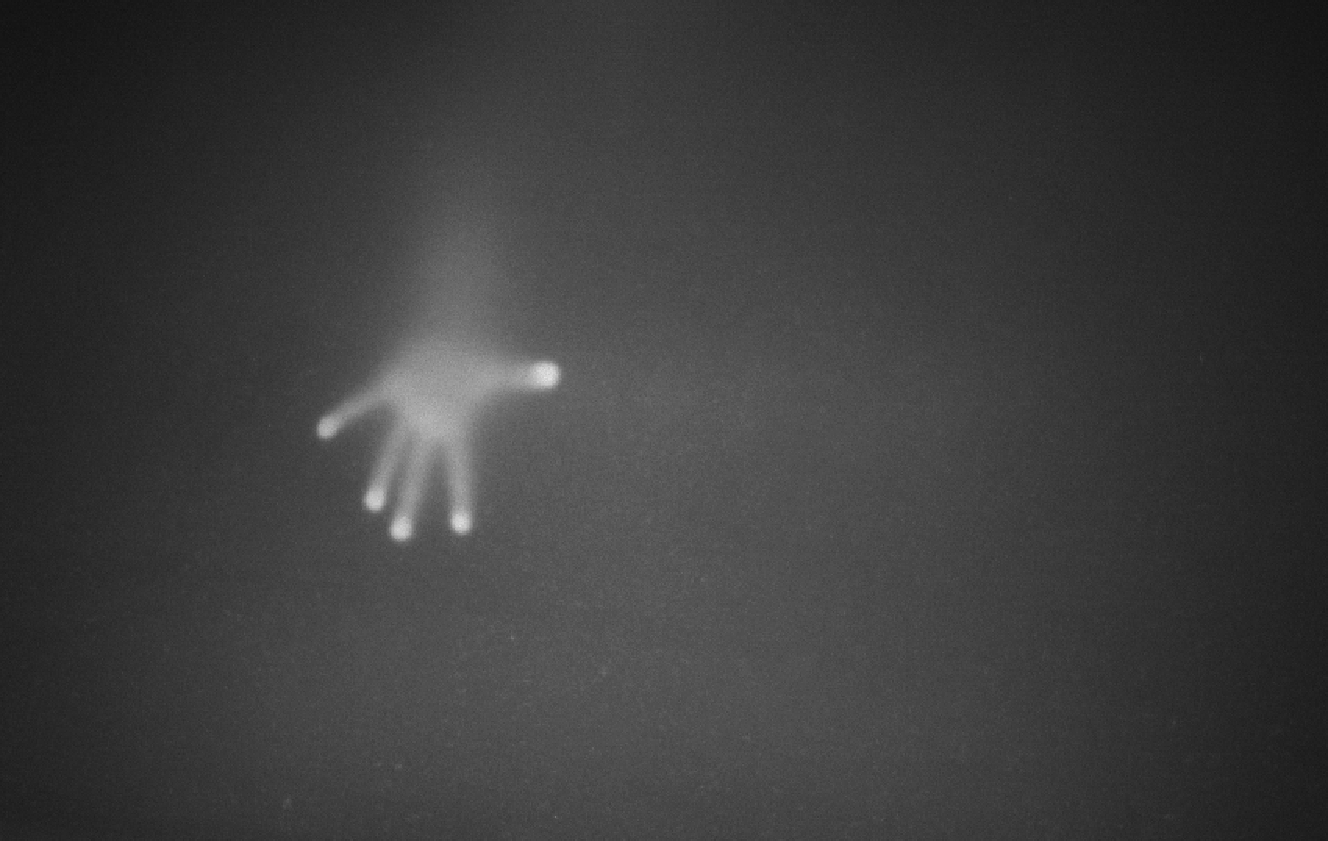
\includegraphics[width=12cm]{img/mser_1.pdf}
	\end{center}
	\caption{Das von der Infrarot Kamera eingefangene Rohbild zur Toucherkennung.}
	\label{fig:mser_1}
\end{figure}

Maximally Stable Extremal Regions ist ein Ansatz entwickelt von Matas et al. zur Auswertung von Bildreihen bei der photogrammetrischen Stereo-Rekonstruktion \cite{matas:2004}. Hierbei sollen vor allem eigenschaftsbezogene Korrespondenzen zwischen Stereobildpaaren mit unterschiedlichem Blickpunkt gefunden werden. Ewerling et al. nutzen diese Erkenntnisse zur Erkennung von Fingerspitzen auf dem Bildschirm \cite{ewerling:2012}. Es erfolgt dabei außerdem eine Zuordnung von Fingern zu Händen durch den \emph{MSER Component Tree}.  Dieses Verfahren ist motiviert durch die visuelle Wahrnehmung des Hand- und Armschattens auf den Bildern, welche durch Tracking mit diffuser Infrarotbeleuchtung erfasst werden (siehe Abbildung \ref{fig:mser_1}).

Extremal Regions (ER) werden als geschlossene Gruppe von Pixeln bezeichnet, welche entweder eine höhere oder eine niedrigere Farbintensität als umliegende Bildpunkte aufweisen. Die ER $R_i$ ist eine Maximally Stable Extremal Region, wenn $R_i$ eine anderen ER ($R_{i-1}$) umschließt und es eine umschließende ER ($R_{i+1}$) für $R_i$ gibt. Es muss folglich $R_{i-1} \subset R_i \subset R_{i+1}$ gelten. Außerdem muss das Stabilitätskriterium ($s_\Delta(i)$) für $i$ ein lokales Minimum erreichen. Folgende Formel beschreibt die Berechnung von $s_\Delta(i)$:
\\\\
$s_\Delta(i) = \frac{ |R_{i+\Delta}| - |R_{i-\Delta}| } { |R_i| }$
\\\\ 
,wobei $\Delta$ eine durch den Anwender definierte Konstante ist.
\\\\
Ewerling et al. nutzen einen erweiterten Ansatz zur Erkennung der MSER in linearer Zeit, nach dem Vorbild von Nistér et al. \cite{nister:2008}. Bei der direkten Verwendung der Methode von Nistér et al. ergibt sich eine hierarchische Struktur zur Beschreibung  aller gefundenen MSER, basierend auf dem Stabilitätskriterium. Genannte Struktur wird als \emph{Component Tree} bezeichnet. Die Konstruktion dieses Component Trees sei jedoch nach Ewerling et al. unvollständig im Hinblick auf für die Beschreibung der Finger-Hand-Relation wichtige ER. Der erweiterte Algorithmus wurde daher entwickelt, um alle verfügbaren ER zu analysieren.
\\\\
Anhand der ER im Component Tree erfolgt die Ableitung der Fingerpositionen und deren Handzuordnung. Hierfür definieren Ewerling et al. zwei grundlegende Regeln:

\begin{enumerate}
\item Die dunkelste und gleichzeitig größte gefundene ER ist der Wurzelknoten des Component Trees
\item Für alle Kind-Eltern Beziehungen in der Struktur gilt, dass die Kindknoten kleiner sind und eine höhere Farbintensität aufweisen
\end{enumerate}

\begin{figure}
	\begin{center}
		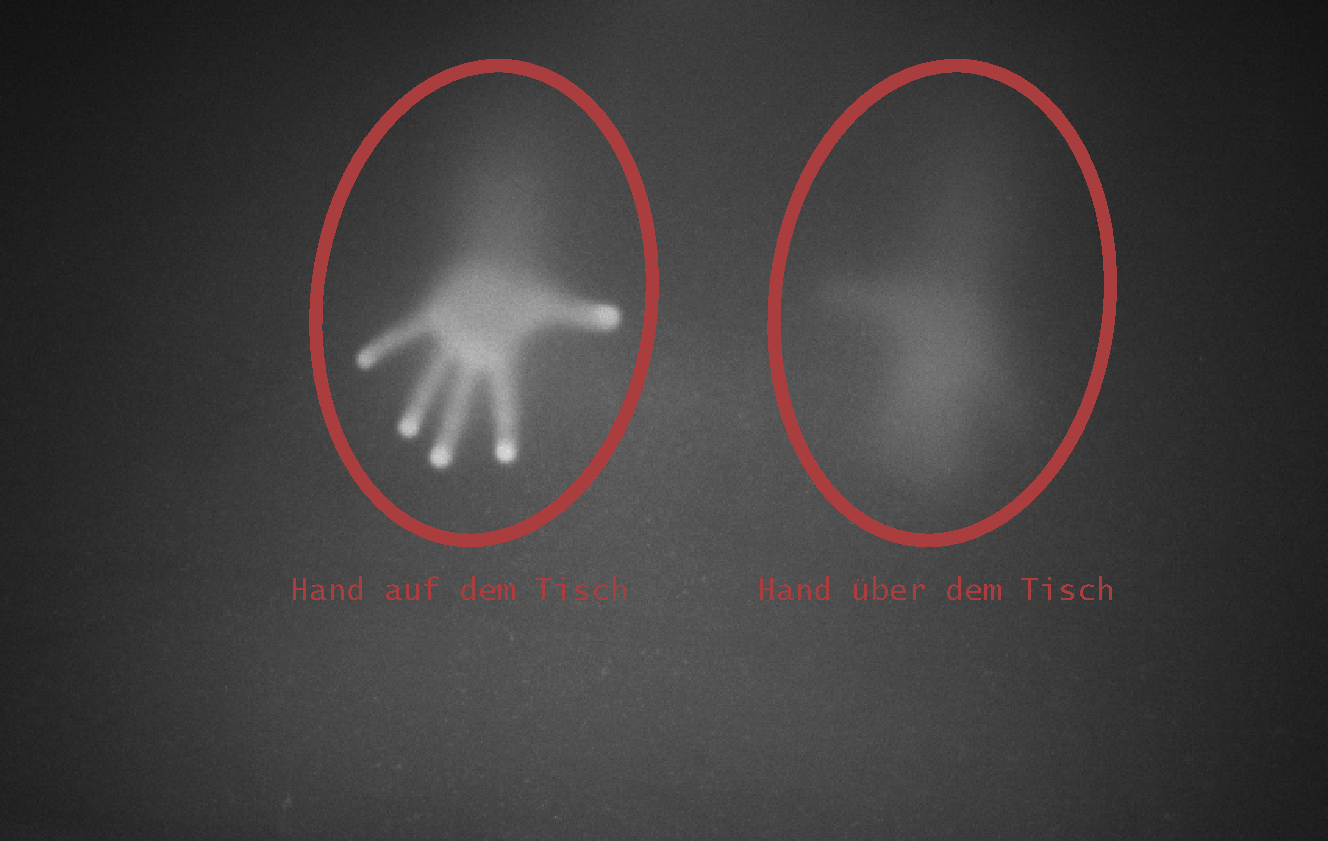
\includegraphics[width=12cm]{img/mser_2.pdf}
	\end{center}
	\caption{Die Helligkeit naher Objekte ist im Infrarot Bild höher als bei weiter entfernten.}
	\label{fig:mser_2}
\end{figure}

Wie in Abbildung \ref{fig:mser_2} zu erkennen ist, kreieren Objekte in naher Distanz zum Bildschirm eine hellere ER als weiter entfernte. Nach den gelisteten Kriterien können folglich nur Blattknoten des Baumes Fingerspitzen sein. Um eine robuste Analyse zu erreichen, werden vermeidliche Kandidaten in der untersten Ebene des Baumes auf typische visuelle Eigenschaften von Fingeraufsetzpunkten getestet. Hierzu zählen das Prüfen auf runde Form und eine definierte Durchschnittsgröße der erkannten Fingerregion. Die Zuordnung der gefundenen Fingerspitzen zu Händen erfolgt über ein hierarchisches Clustering der Knoten im Component Tree.


\section{Technische Voraussetzungen}
\label{sec:technische_voraussetzungen}

Für die technische Umsetzung des in Abschnitt \ref{sec:maximally_stable_extremal_regions} beschriebenen MSER Systems im Kontext der Multi-Touch Erkennung wird in unserem Labor ein rückseitiges, diffuses Infrarot-Beleuchtungssetup genutzt. Hierbei wird eine Infrarot emittierende Lichtquelle unterhalb des Bildschirmtisches angebracht. Diese bestrahlt eine matte und lichtdurchlässige Projektionsfläche. Das von dieser Ebene reflektierte Licht wird durch den Spiegel gelenkt und von einer Infrarotkamera zur weiteren Verarbeitung aufgenommen. Abbildung \ref{fig:table_setup} visualisiert das beschriebene Setup.

\begin{figure}
	\begin{center}
		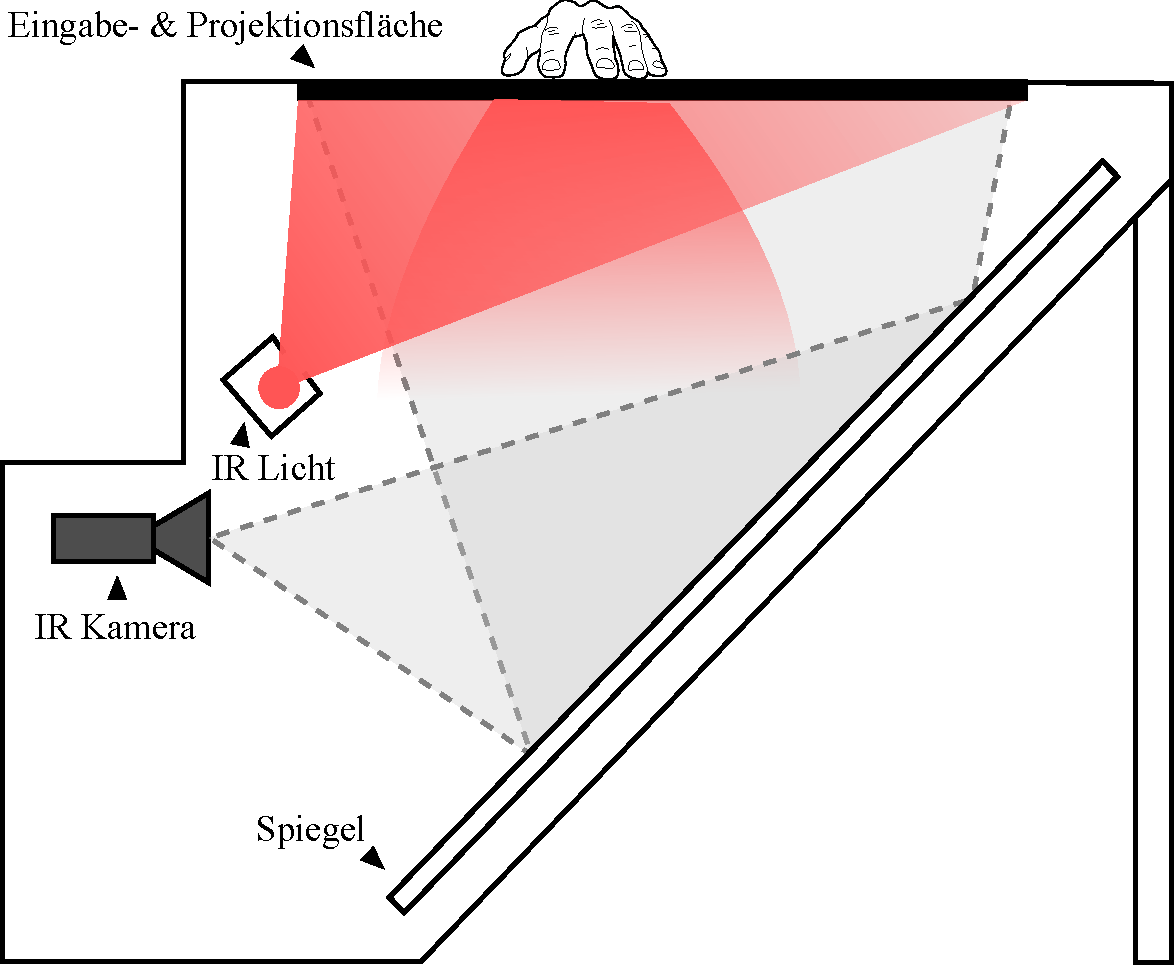
\includegraphics[width=8cm]{img/table_setup.pdf}
	\end{center}
	\caption{Das im Labor verwendete Hardware Setup zum Tracking von Touch Eingaben.}
	\label{fig:table_setup}
\end{figure}

Die Genauigkeit des Systems kann durch infrarotes Umgebungslicht, wie beispielsweise Anteile der Sonnenstrahlung, oder andere im Arbeitsraum befindliche Trackingsysteme, gestört werden. Ewerling et al. schlagen daher eine hochfrequente Modulation der Beleuchtung nach Moeller und Kerne vor \cite{ewerling:2012, moeller:2012}.  Nicht-uniforme Lichtintensität entlang der Tischfläche kann ebenfalls zu Problemen bei der Bildanalyse führen. Diese können zwar durch Filterverfahren abgeschwächt, jedoch nicht vollständig beseitigt werden. Eine gleichmäßige Ausleuchtung der Projektionsebene ist demnach ausschlaggebend für eine akkurate Evaluation der Kamerabilder.


\section{Implementierung}
\label{sec:implementierung_mser}
Es existiert eine Anbindung des MSER Algorithmus zur Touch Erkennung, an das am Lehrstuhl entstandene Applikationsframework Avango \cite{avango:2011}. Die analysierten Eingabedaten werden basierend auf dem TUIO Protokoll an die Anwendung gesendet \cite{tuio}.
\\\\
In Abschnitt \ref{subsec:tuio_touch_protokoll} wird eine Übersicht über die mit dem TUIO Protokoll bereitgestellten Datenstrukturen gegeben. Abschnitt \ref{subsec:umgang_mit_jittering} beschreibt das Auftreten von Jittering bei der Eingabeerkennung und wie mit diesem Problem umgegangen werden kann.


\subsection{TUIO Touch Protokoll}
\label{subsec:tuio_touch_protokoll}

TUIO ist ein von Kaltenbrunner et al. entwickeltes Protokoll, welches speziell für den Umgang mit berührbaren Tabletop Eingabeschnittstellen kreiert wurde \cite{kaltenbrunner:2005}. Nach der Auswertung der Eingabepositionen durch den MSER Algorithmus, füllt die Protokollkommunikation verschiedene Stations im Avango Daemon mit den ermittelten Daten. Es existieren zwei Stationstypen. Der Erste hält Informationen über einen jeweiligen Finger. Dies beinhaltet eine normalisierte Fingerposition und die zugewiesene \emph{SessionID}. Ein weiterer Stationstyp ist für die Verwaltung handspezifischer Details verantwortlich. Hierzu gehören die \emph{SessionID} der Hand, eine Liste von \emph{FingerSessionIDs} der zugewiesenen Finger, sowie eine zweidimensionale Orientierung des Armes. Letztere ist durch die Auswertung der handumschließenden Ellipse gegeben. 
\\\\
Eine Abbildung dieser Struktur ist nach dem Feldcontainer Konzept, welches Avango bereitstellt, in der Applikation umgesetzt. Für jeden der Stationstypen existiert demnach eine Klasse, welche durch Update der Station aktualisierte Eingabewerte für die Anwendung verfügbar macht. Die nachfolgende Abbildung XX zeigt den Aufbau der Klassen \emph{TUIOFinger} und \emph{TUIOHand}.


\subsection{Umgang mit Jittering}
\label{subsec:umgang_mit_jittering}

Die Verfolgung der Bewegung von Eingabepunkten basiert auf der Auswertung von Bilddaten. Hierbei ist die Präzision der Positionsermittlung an die Genauigkeit des MSER Algorithmus, sowie die Auflösung der Bilder gebunden. Infolgedessen können, selbst bei Auflegen eines Fingers ohne Positionsverschiebung, variierende Eingabepositionen entstehen. In einer Visualisierung der Eingabeposition äußert sich dieser Zusammenhang als Zittern (Jittering) der Darstellungsgeometrie.
\\\\
Jittering kann bei Anwendung der Eingabe auf die Manipulation einer virtuellen Szene ungewollte Auswirkungen hervorrufen. Bindet man eine Szene beispielsweise an die relative Positionsänderung einer durch Jittering beeinträchtigten Eingabe, so überträgt sich das Zittern auf die Szene, was als störend für die Wahrnehmung empfunden werden kann. Die Initiierung einer Bewegung sollte folglich weitestgehend dem Anwender überlassen sein.
\\\\ 
Um Jittering zu vermindern wird vor der Übermittlung von Daten durch das TUIO Protokoll ein Filter auf die Eingabepositionen angewandt. Hierzu wird der von Casiez et al. vorgestellte \emph{1\euro{} Filter} verwendet \cite{casiez:2012}. Dieser Ansatz überzeugt vor allem durch seine niedrige Rechenintensität, sowie die geringe Latenzanfälligkeit bei schnellen Bewegungen.


\section{Vorteile und Limitierungen}
\label{sec:diskussion_mser}

Das MSER-System dient zur Erkennung von relationalen Eingabedaten. Es können somit Aussagen über die hierarchische Zuordnung einzelner Fingerpositionen zu aufgelegten Händen gemacht werden. Dieser Zusammenhang ist essenziell für die im Rahmen dieser Arbeit entstandenen Techniken. 
\\\\ 
Im Umgang mit der Toucherkennung wurden im Verlauf der Programmierarbeiten jedoch immer wieder verschiedene Probleme deutlich. Demnach wird eine Finger-Hand Zuweisung zwar unterstützt, nicht konsequent stabil gehalten. Die Variation der Höhe der Handfläche über dem Tisch kann beispielsweise zum Auflösen der Verbindung einzelner Teile der Wurzel ER einer Hand führen. In diesem Fall stellt sich die Eingabe einer Hand mit fünf aufgelegten Fingern, als mehrere Einzelne Hände mit einem Finger dar. 
\\\\
Das gleichzeitige Aufsetzen zweier Hände eines Nutzers wird nur dann problemfrei erkannt, wenn zwei separate ER für die Arme entstehen. Beugt sich der Anwender über die Tischplatte um mit beiden Händen in weit entfernten Bereichen zu interagieren, kann leicht eine Verschmelzung der ER um beide Arme entstehen. Dies beeinträchtigt eine kollisionsfreie Handerkennung weiter. Dementgegen ist die Erkennung und Verfolgung einzelner Eingabepunkte relativ stabil. Lediglich schnelle Bewegungen über die Tischfläche sind hierbei problematisch und führen zum Verlust von Fingerpositionen.

%------------------------------------------------

\chapter{Anforderungsanalyse}
\label{chp:anforderungsanalyse}
Hier wird das Kapitel Anforderungsanalyse beschrieben. Das Kapitel besteht aus den Abschnitten \ref{sec:mehrbenutzer_touch_eingaben}, \ref{sec:tiefenwahrnehmung}, \ref{sec:interaktionsziele_und_freiheitsgrade}, \ref{sec:kontrolle_der_freiheitsgrade} und \ref{sec:visuelle_rueckmeldung}.


\section{Mehrbenutzer Touch-Eingaben}
\label{sec:mehrbenutzer_touch_eingaben}

Hier steht Inhalt zu Mehrbenutzer Touch-Eingaben.


\section{Tiefenwahrnehmung durch Stereo- und Bewegungsparalaxe}
\label{sec:tiefenwahrnehmung}

Hier steht Inhalt zu Tiefenwahrnehmung durch Stereo- und Bewegungsparalaxe. 


\section{Interaktionsziele und involvierte Freiheitsgrade}
\label{sec:interaktionsziele_und_freiheitsgrade}

Hier steht Inhalt zu Interaktionszielen und involvierten Freiheitsgraden. 


\section{Explizite und implizite Kontrolle der involvierten Freiheitsgrade}
\label{sec:kontrolle_der_freiheitsgrade}

Hier steht Inhalt zu Expliziter und impliziter Kontrolle der involvierten Freiheitsgrade.


\section{Visuelle Rückmeldung}
\label{sec:visuelle_rueckmeldung}

Hier steht Inhalt zu Visueller Rückmeldung. 

%------------------------------------------------

\chapter{3D Interaktion mit Multitoucheingaben}
\label{chp:interaktion_mit_multitoucheingaben}
Die Interaktion mit Multi-Touch Eingaben wurde in einigen Veröffentlichungen thematisiert. Hierbei haben sich unterschiedliche Strategien, zur Kontrolle der Freiheitsgrade bei der Manipulation von dreidimensionalen Szenen, bewährt. (!?!?Des Weiteren wurden verschiedene Kriterien entwickelt, welche zur Bewertung von Multi-Touch Techniken dienen!?!?) Die im Rahmen dieser Arbeit entstandenen Ansätze, zur Umsetzung einer Multi-Touch basierten 3D Navigation, stützen sich auf diese Erkenntnisse.
\\\\
Dieses Kapitel stellt die in diesem Kontext wichtigsten verwandten Arbeiten vor. Hierzu beschreibt Abschnitt \ref{sec:related_sticky_tools} ein System zur 6DOF Interaktion mit Multi-Touch Tischen. In Abschnitt \ref{sec:related_balloon_selection} wird ein Ansatz zur Selektion von virtuellen Objekten, durch Touch Eingaben erläutert. Abschnitt \ref{sec:related_two_axis_valuator} erklärt die Umsetzung einer expliziten Geste zur Steuerung der 3D Rotation. Abschließend erfolgt in Abschnitt \ref{sec:diskussion_interaktion} eine Diskussion genannter Techniken.


\section{Sticky Tools}
\label{sec:related_sticky_tools}

Hancock et al. stellen ein System zur Steuerung von sechs Freiheitsgraden der dreidimensionalen Objekttransformation durch Multi-Touch Eingaben vor, welches sie Sticky Tools nennen \cite{hancock:2009}. Sie stützen sich dabei auf bekannte Techniken welche als \emph{force-based} bezeichnet werden. Hierbei soll das Gefühl erzeugt werden, die virtuelle Geometrie wie in der realen Welt durch direktes Anfassen zu manipulieren. 
\\\\
Die x- und y-Translation, uniforme Skalierung, sowie z-Rotation mit zwei Fingern hat sich im Alltag, durch den Umgang mit zweidimensionalen Touch-Anwendungen, bewährt. Es wird hierbei ein Initialkontakt mit der Geometrie bestimmt. Während der Bewegung der Finger, bleibt dieser durch Anwendung der genannten Transformationen, erhalten. Dieses \emph{Ankleben} der Objekte an die Berührungspunkte auf dem Bildschirm bezeichnen Hancock et al. als \emph{Sticky Fingers}-Technik \cite{hancock:2007,hancock:2009}.
\\\\
In dreidimensionalen Szenen wird die Translation um die z-Komponente erweitert. Hancock et al. nutzen für die Visualisierung der virtuellen Szene eine zweidimensionale Darstellung. Durch die perspektivische Verzerrung wächst der projizierte Abstand zweier Punkte auf einem Objekt, je mehr sich die Geometrie der Projektionsebene nähert. Sticky Tools simulieren den physikalischen Umgang mit nicht-elastischen Objekten. Aus diesem Grund wird auf eine Geste zur Skalierung verzichtet. Folglich wird die 2D Skalierungsgeste zur z-Translation eines Objekts genutzt.
\\\\
Neben der Rotation um die Hochachse ermöglicht die Manipulation in dreidimensionalen Szenen das Drehen von Objekten um Achsen auf der Bildfläche. Hancock et al. definieren letztere als \emph{flip}-Rotation. Um das Sticky Fingers Kriterium zu erhalten, wird diese Art der Rotation durch beidhändige Interaktion gesteuert. Hierbei werden durch das Aufsetzen zweier Finger einer Hand die direkten Kontaktpunkte auf der Geometrie festgelegt. Diese spannen einen Richtungsvektor auf, welcher die Rotationsachse definiert. Die Bewegung eines aufgesetzten Fingers der zweiten Hand im rechten Winkel zur Rotationsachse, legt den Grad der Flip-Rotation, sowie die Richtung der Drehung fest (siehe Abbildung \ref{fig:opposable_thumbs}).

\begin{figure}
	\begin{center}
		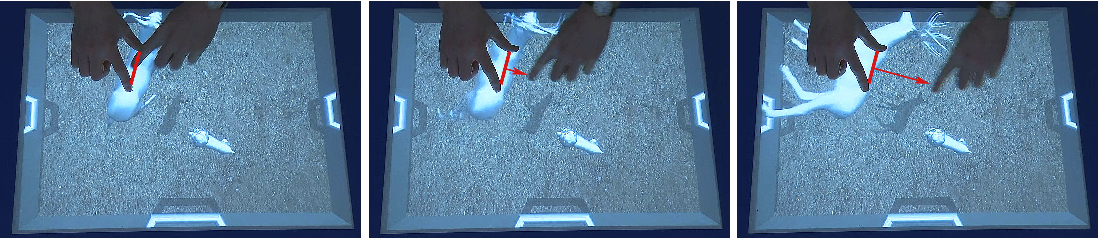
\includegraphics[width=12cm]{img/opposable_thumbs.pdf}
	\end{center}
	\caption{Durchführung der Opposable Thumbs Rotation im von Hancock et al. entwickelten System Sticky Tools \cite{hancock:2009}. Screenshots sind dem zugehörigen Video entnommen und durch eigene Visualisierungen erweitert worden \cite{hancock:2009:vid}.}
	\label{fig:opposable_thumbs}
\end{figure}


\section{Balloon Selection}
\label{sec:related_balloon_selection}

Balloon Selection ist eine von Benko und Feiner \cite{benko:2007} entwickelte Technik zur Multi-Touch basierten Selektion von virtuellen Objekten in dreidimensionalen Szenen. Dieser Ansatz ist inspiriert vom Umgang mit einem Helium Ballon. Demnach wird das Ende der Leine eines solchen Ballons mit einem Finger auf den Boden gehalten. Ein zweiter Finger fixiert die Leine an einem anderen Punkt auf dieser Ebene. Die Länge des fixierten Stückes bestimmt die Aufstiegsdistanz des Ballons. Folglich kann diese Distanz, sowie die Position des Ballons über dem Boden, durch das Verschieben der Handpositionen variiert werden. Abbildung XX visualisiert diese Metapher.
\\\\
Bei der Anwendung dieser Idee für die Selektion, wird eine Kugel als Selektionsobjekt genutzt. Die abgeleitete Geste wird durch das Aufsetzen zweier Finger in unmittelbarer Nähe zueinander initiiert. Hierbei dient der zuerst aufgelegte Finger als Ankerpunkt (nach Benko und Feiner \emph{anchor}). Der zweite Finger (nach Benko und Feiner \emph{stretching finger}) wird zur Festlegung der Leinenlänge verwendet. Hierzu bewegt der Nutzer seine Hand vom Ankerpunkt weg. Die Interaktionsleine wächst bis diese Bewegung sich in entgegen gesetzte Richtung umkehrt. Ab diesem Punkt ist die Länge der Leine fest und die Kugel steigt um die Länge der Distanzverkürzung zwischen den beiden Fingern orthogonal zur Tischebene nach oben. Der Ankerpunkt bestimmt durch Positionsveränderung die x- und y- Position des Ballons über der Interaktionsfläche (siehe Abb XX.).


\section{Two Axis Valuator}
\label{sec:related_two_axis_valuator}

Rousset et al. beschreiben eine Erweiterung von Scheurich und Stuerzlingers \emph{Two Axis Valuator} (im Folgenden TAV genannt) \cite{scheurich:2013,rousset:2014}. Der von Elisabeth Rousset et al. entwickelte TAV+ ist ein Modus zur einhändigen 3D Rotation durch die Verwendung von zwei Fingern. 
\\\\
Für die Bestimmung der Rotation entlang einer beliebigen Achse auf der Bildebene, wird die Bewegung der Zentrumsposition zwischen den aufgesetzten Fingern verfolgt. Die Rotation wird hierbei um die Achse, welche rechtwinklig zur Bewegungsrichtung steht und ebenfalls in der Bildebene liegt, durchgeführt. Als Rotationszentrum dient der Schwerpunkt des zu manipulierenden Objekts. Drehrichtung und Rotationsgrad werden von der Distanz und Richtung der Translation des Fingerzentrums abgeleitet. Zusätzlich kann die Rotation um die Achse zwischen Fingerzentrum und Rotationszentrum kontrolliert werden. Dies ist durch Orientierungsänderung des Vektors zwischen den Fingern möglich. Der verwendete Winkel, entspricht dem zwischen dem Vektor, vor der Bewegung und demselben danach. Abbildung \ref{fig:tav_plus} illustriert das Verfahren.

\begin{figure}
	\begin{center}
		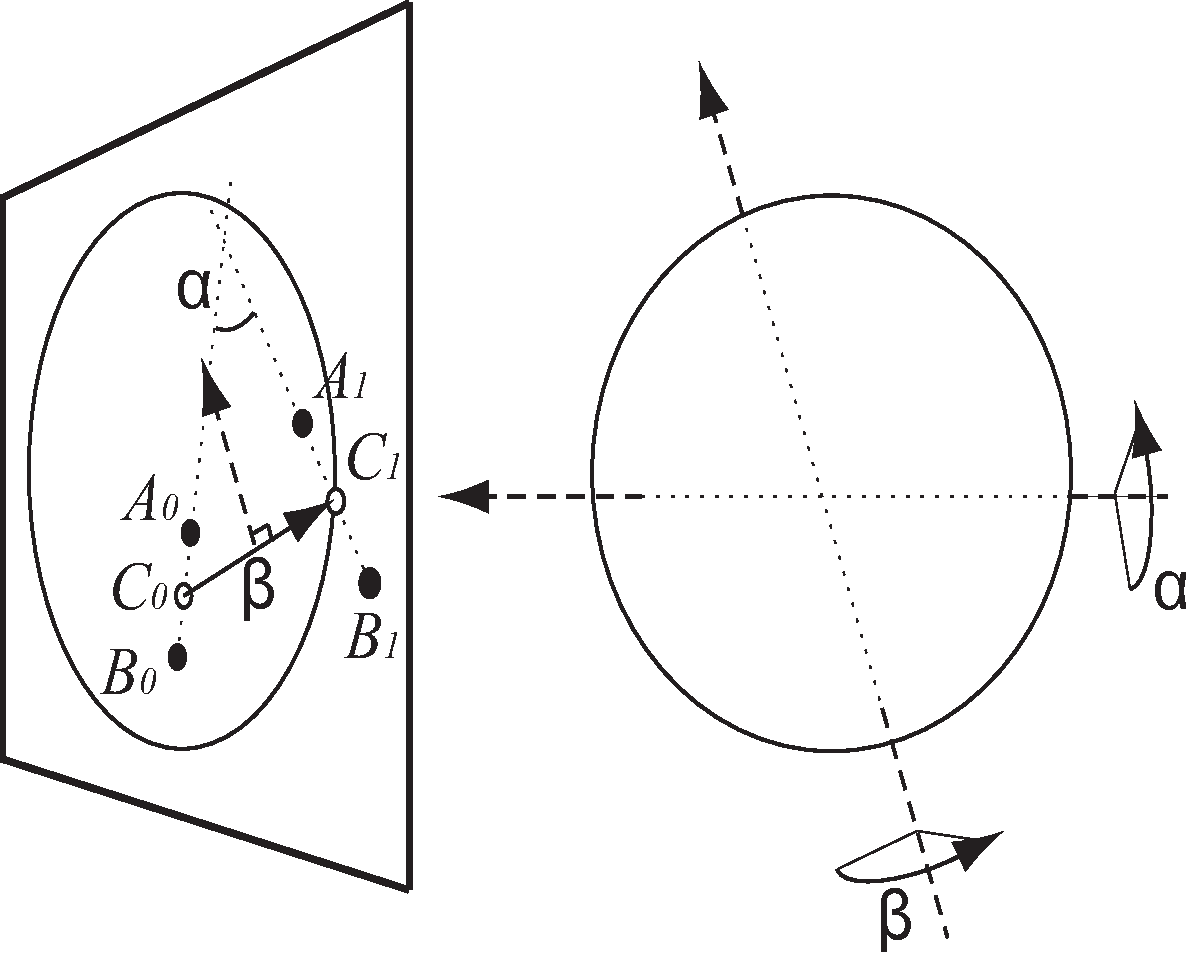
\includegraphics[width=10cm]{img/tav_plus.pdf}
	\end{center}
	\caption{Berechnung der dreidimensionalen Rotation TAV+ nach Rousset et al. \cite{rousset:2014}. Hierbei sind $A_i$ und $B_i$ die zwei zur Interaktion verwendeten Finger. $C_i$ ergibt sich als die Zenntrumsposition zwischen $A_i$ und $B_i$. $\alpha$ und $\beta$ sind die durch das Verfahren ermittelten Rotationswinkel. Diese Abbildung entstammt vollständig einer Veröffentlichung von Rousset et al \cite{rousset:2014}.}
	\label{fig:tav_plus}
\end{figure}


\section{Diskussion}
\label{sec:diskussion_interaktion}

Der direkte Umgang mit negativ-parallaxen Inhalten zeigt sich bei Touch-Interaktion mit stereoskopischen Visualisierungen als problematisch. Benko und Feiner kommen zu dem Schluss, dass Baloon Selection ein unter verschiedenen Umständen geeigneter Ansatz zur Selektion von über einer Interaktionsoberfläche liegenden virtuellen Objekten ist \cite{benko:2007}. Eine Umkehrung der Selektionsrichtung könnte das Verfahren auch für die 3D Multi-Touch Interaktion sinnvoll einsetzbar machen. Die Selektion von virtuellen Inhalten wird im Kontext dieser Arbeit nicht betrachtet. Jedoch ist eine explizite Höhenanpassung der Navigation, basierend auf den Erkenntnissen von Benko und Feiner, entstanden. Diese wird in Abschnitt \ref{sec:3d_translation} näher erläutert.
\\\\
Sticky Tools zeigen sich durch ihre physikalisch motivierte Entwicklung als intuitiv und nutzerfreundlich für die 3D Objektmanipulation.
\\\\
???CITE???
\\\\
Aus diesem Grund fließen einige der von Hancock et al. entwickelten Konzepte maßgeblich in die entstandene 3D Multi-Touch Navigation ein. Sticky Tools ersetzen die Funktionalität der herkömmlichen 2D Skalierungsgeste mit einer expliziten Höhenanpassung. Durch die perspektivische 2D Projektion geht hierbei visuell die direkte Verbindung zu den Kontaktpunkten auf der Geometrie nicht verloren. Stereoskopisches Rendering kann diese Illusion jedoch nicht gewährleisten. Zum Erhalt der Orthogonalität ist in diesem Anwendungsszenario eine uniforme Skalierung unabdingbar. 
\\\\
Der Umgang mit Objekten ist bei Sticky Tools auf geringe Entfernungen zur Bildebene begrenzt. Durch das Aufsetzen zweier Finger auf die Touch-Fläche werden Referenzpunkte auf der Geometrie festgelegt. Aus diesen Punkten wird eine Achse für die flip-Rotation abgeleitet. Weisen die Referenzpunkte einen Höhenunterschied auf, so wirkt sich dieser auf die hervorgerufene Drehung aus. Auf nahe Distanz zu manipulierenden Inhalten, ist die Höhendifferenz gut abschätzbar. Im Umgang mit komplexen Miniaturwelten und bei möglichen weiten Distanzen zu Objekten, wird diese Abschätzung zunehmend schwerer. Es ist in diesem Kontext von einer Beeinträchtigung der Nutzbarkeit der flip-Rotation auszugehen.
\\\\
TAV+ wird von Rousset et al. als 3D Rotationstechnik, welche für unerfahrene Nutzer einfach bedienbar ist, bewertet. Im direkten Vergleich mit anderen 3D Rotationstechniken schneidet TAV+ gut ab. Hierbei wird der Ansatz im Szenario einfacher Observationsaufgaben einzelner Objekte mit fester Position untersucht. Die Wahl des Rotationszentrums im Schwerpunkt der Geometrie erscheint in diesem Zusammenhang als sinnvoll. Bei der Navigation wird der Blickpunkt auf die Szene und somit alle virtuellen Objekte fortlaufend geändert. In diesem Fall wäre die Bedienung der TAV+ Rotation mit festem Rotationsreferenzpunkt sicherlich wenig nützlich. Abschnitt \ref{sec:3d_rotation} beschreibt wie der von Rousset et al. entwickelt abgeändert wurde, um einen effektive 3D Rotation der Navigation zu erreichen.


%------------------------------------------------

\chapter{Wahrnehmungskonflikte und Lösungsansätze}
\label{chp:wahrnehmungskonflikte_und_loesungsansaetze}
Die Darstellung virtueller Szenen durch stereoskopisches Rendering erzeugt die Illusion, dass projizierte Inhalte unter, auf oder über der Bildschirmfläche liegen. Eine konfliktfreie Wahrnehmung der Visualisierung kann durch verschiedene Faktoren eingeschränkt werden. Multi-Touch Eingaben wirken sich durch direkten Kontakt mit dem Projektionssystemen zusätzlichen auf bestehende Probleme aus. In diesem Kapitel werden einige der hervorgerufenen Wahrnehmungskonflikte vorgestellt. Zusätzlich werden bestehende Lösungsansätze aufgezeigt.
\\\\
Abschnitt \ref{sec:related_frame_cancellation} führt hierzu in die Thematik \emph{Frame Cancellation} ein. In Abschnitt \ref{sec:related_touch_interaktion_stereo} werden Probleme und Lösungsbestrebungen beschrieben, welche aufgrund von Touch Interaktion mit stereoskopischen Visualisierungen entstehen. Das Kapitel wird in Abschnitt \ref{sec:diskussion_wahrnehmungskonflikte} durch eine Diskussion dieser verwandten Arbeiten abgeschlossen.


\section{Frame Cancellation}
\label{sec:related_frame_cancellation}

\emph{Frame Cancellation} ist ein Problem, welches in den frühen Jahren der stereoskopischen Filmproduktion von Valyus und Asher erstmals öffentlich benannt wurde \cite{valyus:1966}. Der Wahrnehmungskonflikt entsteht durch eine auftretende Widersprüchlichkeit des Tiefeneindrucks an den Begrenzungen der Projektionsfläche. Bei der Darstellung negativ-parallaxer Inhalte vermittelt die Disparität der Geometrie demnach, dass sich die Darstellung vor dem Bildschirm befindet. Gleichzeitig überlagert dieser durch seine physikalische Begrenzung das Objekt. 
\\\\
Wartell beschreibt eine durch \emph{Frame Cancellation} entstehende schwache Tiefenwahrnehmung der Szene \cite{wartell:2001}. Nach Lipton resultiert außerdem ein unangenehmer visueller Eindruck, durch die Schwierigkeit die Bilder der beiden Augen zu vereinigen \cite{lipton:2007}. 
\\\\
Zum Umgang mit diesem Problem, schlägt Autodesk die Verwendung von \emph{Black Bands} vor \cite{autodesk:2008}. Nach diesem Ansatz werden an den äußeren Begrenzungen des Bildes, der jeweiligen Augen schwarze Balken eingeschoben. Abbildung \ref{fig:black_bands} zeigt, dass ohne Anwendung der Technik im Bild des rechten Auges ein kleinerer Ausschnitt der Geometrie zu sehen ist als im rechten. Dieser fehlende Ausschnitt im Bild des linken Auges führt zum beschriebenen Konflikt. Durch Einschieben der \emph{Black Bands} soll die konfliktfreie Verschmelzung der von beiden Augen wahrgenommenen Bilder ermöglicht werden. 

\begin{figure}
	\begin{center}
		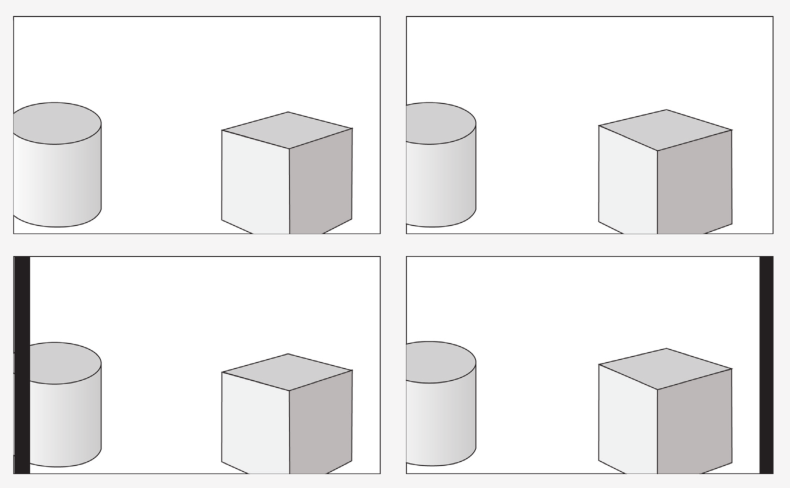
\includegraphics[width=10cm]{img/black_bands.pdf}
	\end{center}
	\caption{Die oberen Abbildungen zeigen die Bildausschnitte der Augen vor Anwendung der \emph{Black-Bands} Technik nach Autodesk \cite{autodesk:2008}. In den darunter liegenden Abschnitten ist die Veränderung dieser nach der Verwendung des Ansatzes zu sehen. Diese Abbildung entstammt vollständig einer Veröffentlichung von Autodesk \cite{autodesk:2008}.}
	\label{fig:black_bands}
\end{figure}

Ardouin et al. schlagen die Verwendung von Clipping zur Begrenzung des Blick Frustums vor \cite{ardouin:2011}. Der Schnittbereich der Frusta beider Augen wird nach Ardouin \emph{Stereo Compatible Volume} genannt \cite{ardouin:2011}. In diesem Bereich sei eine konfliktfreie Visualisierung negativ-parallaxer Szeneninhalte sicher. Das Abschneiden der Geometrie außerhalb des Stereo Compatible Volumes (nach Ardouin \emph{Stereo Compatible Volume Clipping}) würde demnach \emph{Frame Cancellation} vermeiden. Abbildung \ref{fig:scvc} zeigt eine Gegenüberstellung der Technik von Ardouin et al. mit \emph{Black-Bands}.

\begin{figure}
	\begin{center}
		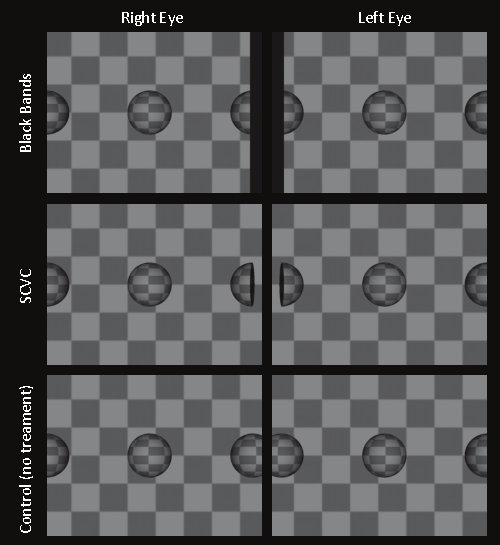
\includegraphics[width=8cm]{img/black_bands_and_SCVC.pdf}
	\end{center}
	\caption{Gegenüberstellung der Techniken \emph{Stereo Compatible Volume Clipping} nach Ardouin et al \cite{ardouin:2011} und \emph{Black-Bands} nach Autodesk \cite{autodesk:2008}. Zum Vergleich wird eine unveränderte Darstellung der Bildausschnitte gezeigt. Diese Abbildung entstammt vollständig einer Veröffentlichung von Ardouin \cite{ardouin:2011}.}
	\label{fig:scvc}
\end{figure}


\section{Touch Interaktion mit stereoskopischen Visualisierungen}
\label{sec:related_touch_interaktion_stereo}

Bei der Touch Interaktion ist die Selektion und Manipulation von virtuellen Objekten auf und abseits der Projektionsebene ausschließlich durch Eingaben auf der Tischebene zu erreichen. Daraus leitet sich eine Wahrnehmungsdiskrepanz ab \cite{valkov:2011,bruder:2013}. Demnach ist die Wahl des Fokuspunktes für die Beobachtung des Interaktionsvorgangs doppeldeutig. Ein Objekt in Negativ- Parallaxe liegt oberhalb der Tischebene, sodass bei Fokussierung von selbigem die Blickrichtung der beiden Augen über der Projektionsfläche konvergiert. Die Wahrnehmung der interagierenden Hand auf dem Bildschirm würde folglich verschwimmen. Umgekehrt würde die Wahrnehmung des parallaxen Inhalts bei Fokussierung der Hand verschwimmen. Abbildung \ref{fig:fokussierung} verdeutlicht diesen Zusammenhang.

\begin{figure}
	\begin{center}
		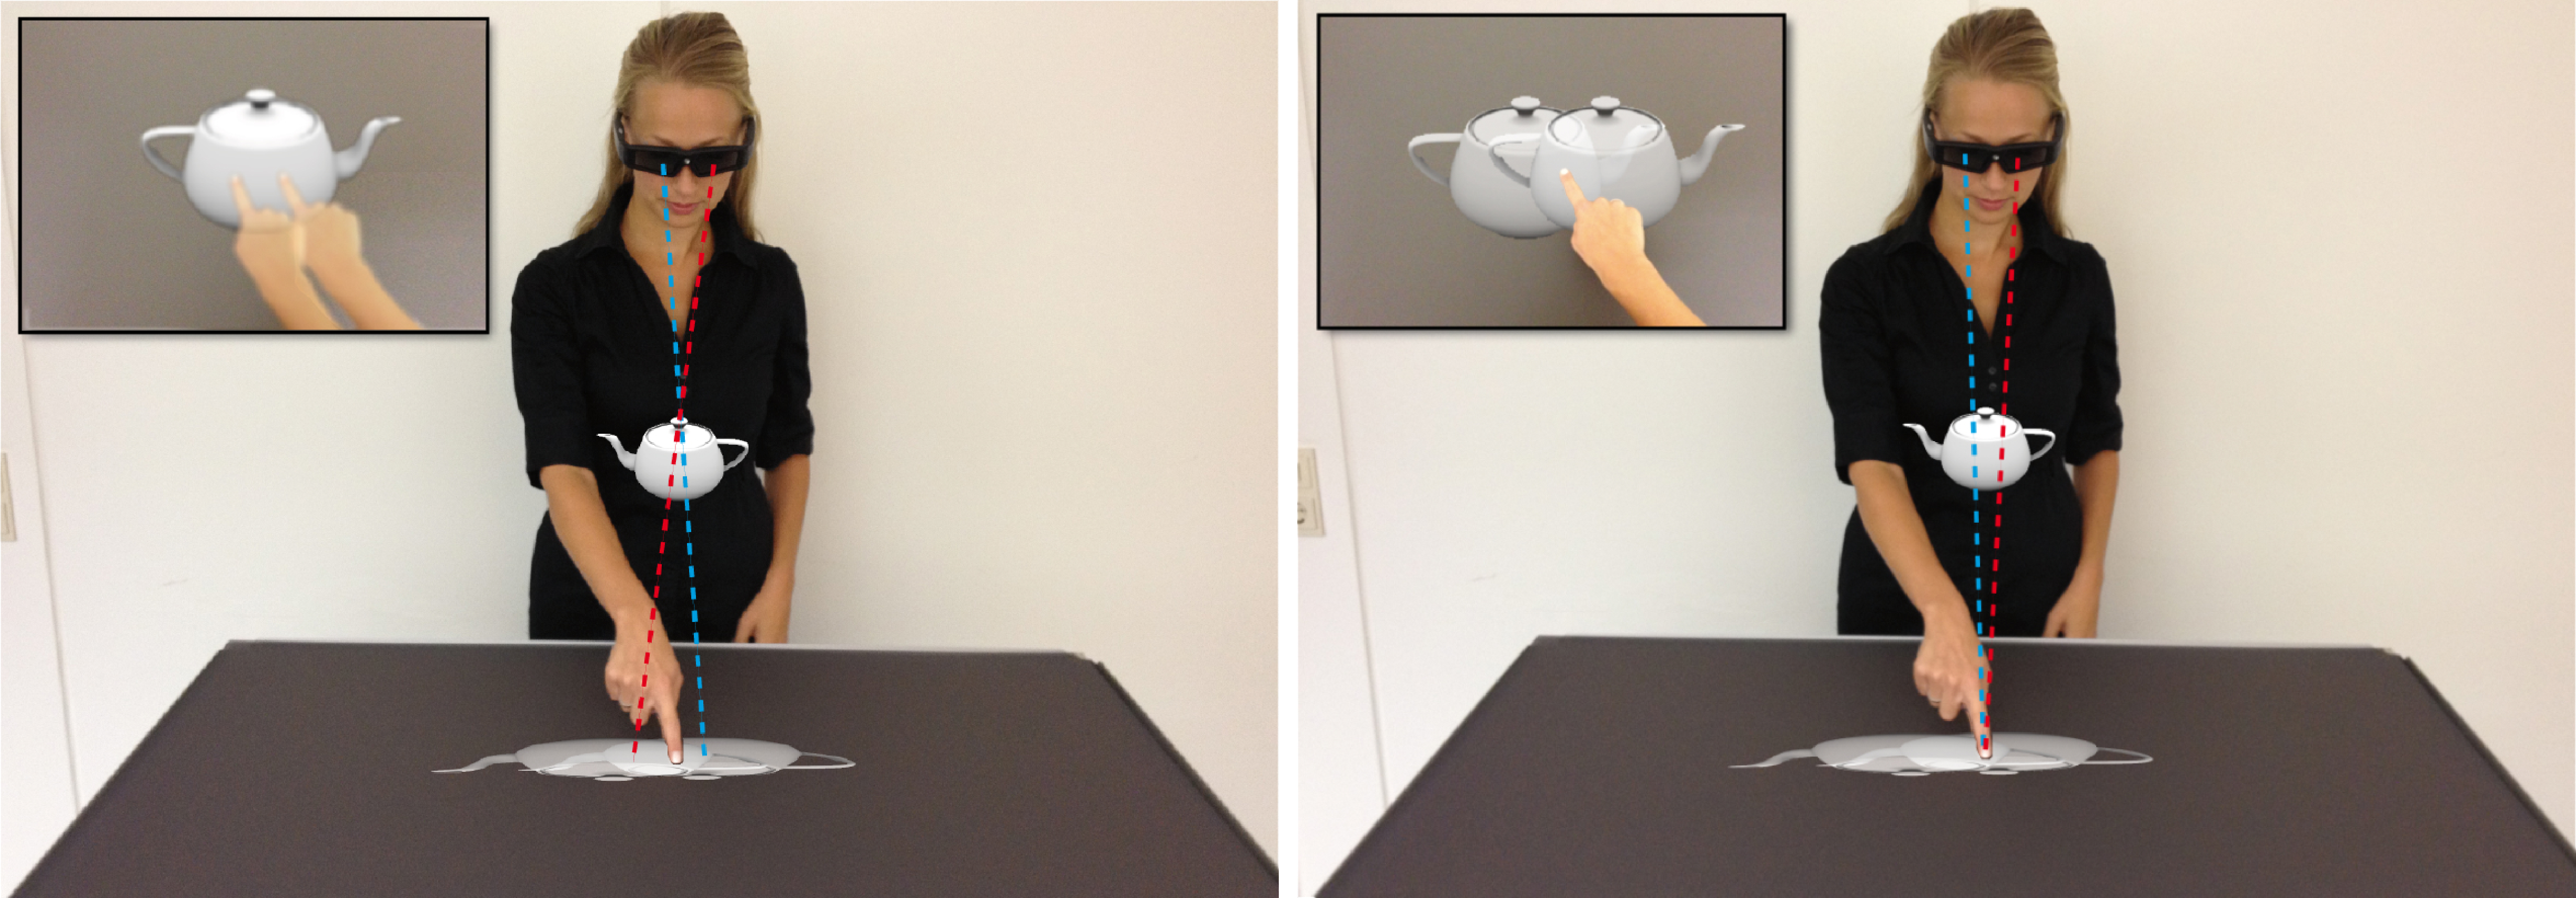
\includegraphics[width=12cm]{img/fokussierung.pdf}
	\end{center}
	\caption{Wahrnehmungsdiskrepanz durch die Wahl des Fokuspunkts. Diese Abbildung entstammt vollständig einer Veröffentlichung von Bruder et al. \cite{bruder:2013}.}
	\label{fig:fokussierung}
\end{figure}

Giesler et al. entwickeln mit ihrer Technik \emph{Void Shadows} einen Ansatz um die Touch Selektion von nicht auf der Bildfläche liegenden Objekten zu erleichtern \cite{giesler:2014}. Hierzu wird eine zweidimensionale Repräsentation aller Geometrie als Schatten auf die Bildebene projiziert. Berührungen eines Schattens werden auf die jeweilig referenzierte Geometrie übertragen.
\\\\
Ein weiteres Problem ergibt sich durch das Eindringen der Hand in über dem Tisch liegende Geometrie. Berührt der Anwender die Tischebene zur Interaktion, durchstößt er dabei die auf dem Pfad der Bewegung liegenden negativ-parallaxen Objekte. Während dem Nutzer durch die Disparität der Darstellung eine geometrische Lage der Inhalte oberhalb der Hand suggeriert wird, bleiben diese verdeckt bis die Hand des Nutzers die Eingabefläche verlässt. Folglich wird die Tiefenwahrnehmung durch die widersprüchliche Lage des projizierten Inhalts in Relation zur Hand des Nutzers gestört. Hierdurch wird der visuelle Eindruck wie bei \emph{Frame Cancellation} (siehe Abschnitt \ref{sec:related_frame_cancellation})  beeinflusst.
\\\\
Um dieser Problematik entgegenzuwirken verfolgt das von de la Rivière et al. entwickelte System die Bewegung der Hand Nutzer über dem Tisch \cite{delariviere:2010}. Nähert sich diese der Tischfläche, wird die Szene entlang der Bildschirmnormalen in Blickrichtung des Nutzers verschoben, bis alle virtuellen Inhalte auf oder unter der Projektionsfläche liegen. Sie verhindern somit mögliche Kollisionen der Hand mit allen dargestellten Objekten.


\section{Diskussion}
\label{sec:diskussion_wahrnehmungskonflikte}

Stereoskopisch Projektionssysteme erzeugen durch physikalisch motiviertes Rendering die Illusion einer tatsächlichen Dreidimensionalität der dargebotenen Inhalte. Die in Abschnitte \ref{sec:related_frame_cancellation} und \ref{sec:related_touch_interaktion_stereo} zeigen jedoch, dass die Form der Darstellung, sowie der direkte Umgang mit projizierten Inhalten zu verschiedenen Wahrnehmungskonflikte führen können. Es entsteht dadurch eine Herausforderung für die nutzerfreundliche Zusammenführung mit einem an die zweidimensionale Tischfläche gebundenen Multi-Touch System. 
\\\\
Für die Lösung des \emph{Frame Cancellation} Problems wurde eine Reihe von Ansätzen vorgestellt, welche als sinnvolle Lösungen des Problems zu sehen sind (siehe Abschnitt \ref{sec:related_frame_cancellation}). Die Klärung der von Valkov et al. beschrieben Wahrnehmungsdiskrepanz (siehe Abschnitt \ref{sec:related_touch_interaktion_stereo}) bei Fokussierung von negativ-parallaxen Objekten in Relation zur auf dem Tisch aufgelegten Hand bleibt fraglich.
\\\\
In einer Studie vergleichen Burder et al. die Präzision der 3D Selektion bei Verwendung von 2D Touch Eingaben, mit der freien Auswahl im dreidimensionalen Raum (\emph{3D mid-air} Selektion) \cite{bruder:2013}. Sie kommen zu dem Schluss, dass durch \emph{3D mid-air} Selektion eine höhere Genauigkeit mit schnelleren Interaktionszeiten für Objekte, welche weiter als 10cm abseits der Bildebene liegen, gegeben ist.
\\\\
Die fehlende Effizienz von 2D Touch Eingaben, gegenüber \emph{3D mid-air} Techniken könnte durch Ansätze wie \emph{Void Shadows} verbessert werden. Giesler et al. belegen, dass ihre Technik die Präzision und Interaktionszeit, beim Umgang mit vom Bildschirm entfernten Objekten, deutlich verbessert \cite{giesler:2014}. Das Anwendungsszenario beschränkt sich bei ihrer Arbeit auf den Umgang mit positiv-parallaxen Inhalten und sollte für Inhalte oberhalb der Tischeben erweitert werden.
\\\\
Die im System von de la Rivière et al. integrierte Funktionalität beseitigt das Auftreten von Wahrnehmungskonflikten durch Eingreifen in virtuelle Modelle \cite{delariviere:2010}. Folgende Kritikpunkte scheinen jedoch naheliegend:

\begin{itemize}
	\item Der eigentliche Wahrnehmungskonflikt wird nicht gelöst. Man vermeidet lediglich die Konfrontation.
	\item Die Translation der Szene ohne direkte Eingabe des Anwenders ist fraglich für die Nutzerfreundlichkeit des Systems.
	\item Das System erlaubt nicht den Umgang mit der Szene in jeder geometrischen Lage
\end{itemize}

%------------------------------------------------

\chapter{Abbildung von Touch Eingaben in der Applikationsstruktur}
\label{chp:applikationsstruktur}
In den Kapiteln \ref{chp:explizite_interaktion} und \ref{chp:implizite_navigation} werden einige Techniken vorgestellt, welche im Rahmen der Arbeit in einem neuartigen System zur Multi-Touch 3D Navigation vereinigt wurden. Durch die in Kapitel \ref{chp:wechsel_zwischen_interaktionstechniken} eingeführten Ansätze können diese Modular ausgewählt und bedient werden. Zusätzlich erfolgt die Verwendung der \emph{See-Through} Technik (sieh Kapitel \ref{chp:freischneiden}). Hierdurch werden Wahrnehmungskonflikte abgeschwächt, welche durch Eindringen der Hand des Nutzers in Negativ-Parallaxe hervorgerufen werden.
\\\\
In diesem Kapitel wird die Einbindung dieser Konzepte in eine generische Applikationsstruktur präsentiert. Hierzu wird in Abschnitt \ref{sec:multitouch_input_pipeline} die Verarbeitung der vom TUIO Protokoll (siehe Unterabschnitt \ref{subsec:tuio_touch_protokoll}) gelieferten Eingabedaten vorgestellt. Abschnitt \ref{sec:touch_navigation} erklärt den Aufbau und die Arbeitsweise der Touch Navigation als Applikationsmanipulator. In Abschnitt \ref{sec:rep_im_szenegraph} wird die Abbildung der visuellen Repräsentation von Touch Eingaben im Szenegraph beschrieben. Zuletzt werden die in diesem Kapitel dargebotenen Zusammenhänge in Abschnitt \ref{sec:diskussion_applikationsstruktur} auf ihre Vorteile und Limitierungen untersucht.  

\section{Multi-Touch Input Pipeline}
\label{sec:multitouch_input_pipeline}

Die Verarbeitung von Touch Eingaben erfolgt in drei wesentlichen Schritten. Schritt 1 wird einmalig zu Applikationsstart ausgeführt. Hierbei wird für die Maximalanzahl an gleichzeitig erkennbaren Händen jeweils ein Touchwerkzeug angelegt. Während der MSER-Algorithmus (siehe Kapitel \ref{chp:mser}) zur Erkennung von Eingaben keine Begrenzung aufweist, sind die in der Applikation nutzbaren Inputpositionen durch die Anzahl verfügbarer \emph{Stations} im \emph{Avango Daemon} begrenzt (siehe Unterabschnitt \ref{subsec:tuio_touch_protokoll}). Touchwerkzeuge sind vom Anwender konfigurierbar und sollen die Verbindung zwischen der taktilen Eingabe und der jeweiligen Auswirkung dieses Inputs in der Applikation herstellen. Jedes Touchwerkzeug verarbeitet den Input genau einer Hand. Des Weiteren verfügt jedes dieser Werkzeuge über verschiedene Geometrien zur Visualisierung der Eingabe. Der Input einer Hand wird als Teil des Touchwerkzeugs in einem Datencontainer gehalten, welcher bei Bedarf in Schritt 2 gefüllt wird.
\\\\
Sobald durch den in Abschnitt MSER-Algorithmus Fingerkontaktpunkte ermittelt wurden, folgt Schritt 2. An dieser Stelle werden die Daten aus dem TUIO Protokoll Transfer ausgewertet und umstrukturiert. Hierzu werden die angesprochenen Datencontainer gefüllt. Diese identifizieren jede erkannte Hand und enthalten außerdem eine Liste mit Positionen der einzelnen Finger, sowie eine errechnete Handzentrumsposition. Die Handzentrumsposition entspricht dem Mittelpunkt der um alle enthaltenen Finger gespannten Bounding Box. Durch die in Abschnitt \ref{sec:diskussion_mser} vorgestellten Komplikationen bei der Handerkennung, werden Finger nur beim ersten Aufsetzen auf die Tischplatte einer Hand zugewiesen. Bei der Eingabeverfolgung bleibt diese Zuordnung erhalten.
\\\\
Da jeder der in Schritt 2 beschriebenen Datencontainer an ein Touchwerkzeug gebunden ist, erfolgt in Schritt 3 zuletzt die Verknüpfung der Eingabe mit der jeweiligen Auswirkung in der Applikation. Hierzu verfügen Touchwerkzeuge über einen Selektionsmechanismus, welcher basierend auf den vorliegenden Eingabedaten und dem aktuellen Applikationsstatus Kontakt zu einem Applikationsmanipulator herstellt. Dieser wird über Strahlenschnitttests realisiert.


\section{Touch Navigation}
\label{sec:touch_navigation}

Touchwerkzeuge verfügen nicht über die Macht direkte Veränderungen an der Applikation vorzunehmen, ausgenommen der Darstellung ihrer eigenen geometrischen Repräsentation. Sie stellen lediglich durch die gegebenen Input Daten einen Kontakt zu Applikationsmanipulatoren her. Wir definieren diese Manipulatoren als Objekte zur funktionsspezifischen Änderung bestimmter Eigenschaften der Anwendung.
\\\\
Die Touch Navigation ist ein Applikationsmanipulator zur Umsetzung der vorgestellten Multi-Touch Techniken auf die Transformation des virtuellen Bildschirms. Die Klasse benötigt zur Bestimmung der Interaktion Eingabedaten, welche wiederum von den Touchwerkzeugen geliefert werden. Jedes dieser verfügt über einen Selektionsmechanismus, welcher genutzt wird um Kontakt zu Applikationsmanipulatoren wie auch der Touch Navigation aufzubauen. Diese verfügt über eine durchsichtige Geometrie, welche an den physikalischen Bildschirm angehängt wird. Sie referenziert dadurch den für die Eingabe nutzbaren Bereich. Beim Aufsetzen einer Hand wird das zugewiesene Touchwerkzeug aktiviert und führt zwei Strahlenschnittteste aus. Der erste bestimmt den Auftreffpunkt auf der sichtbaren Szenengeometrie. Durch den zweiten Schnitt wird funktionale Geometrie getestet. Dies schließt die Fläche, welche durch die Touch Navigation definiert wurde, sowie etwaige Menüelemente ein. Neben einer Auftreffposition bietet der Schnitt mit funktionaler Geometrie auch die Referenz auf eine bestimmte Klasse. Auf diese Weise kann das Touchwerkzeug durch Schnitt der durchsichtigen Fläche auf dem Bildschirm Zugriff auf die Touch Navigation erhalten.
\\\\
Jeder Applikationsmanipulator ist mit den Funktionen \emph{addContact} und \emph{removeContact} ausgestattet. Nachdem das Touchwerkzeug eine funktionale Geometrie getroffen hat, wird auf der Referenzierten Klasse \emph{addContact} aufgerufen. Diese Funktion wird mit den Eingabedaten des Touchwerkzeugs, einer eindeutigen Identifikationsnummer (ID) für die Bindung, sowie dem Geometrieschnitt des Szeneninhalts parametrisiert. Wird der Kontakt von der Touch Navigation entgegengenommen, speichert das Werkzeug die Bindung und leitet etwaige Veränderungen des eigenen Inputs über \emph{addContact} an den Manipulator weiter. Andernfalls gilt der gegebene Input als blockiert und das Touchwerkzeug hat keine Auswirkung auf die Navigationsinteraktion. Um an den Manipulator gebunden werden muss sich ein gebundener Kontakt lösen und das Touchwerkzeug erneut anmelden. Letzteres ist nach Lösen eines gebundenen Kontakts durch erneutes Aufsetzen der Hand möglich. Da die Touchwerkzeuge keinem Nutzer zugeordnet werden können, wird auf diese Weise die gleichzeitige Interaktion mehrerer Nutzer eingeschränkt. Verliert ein Werkzeug durch Anheben der jeweiligen Hand die Eingabe, so wird der Kontakt durch \emph{removeContact} parametrisiert durch seine zugehörigen ID, von der Navigation abgemeldet. Dieser Zyklus wird in Abbildung XX grafisch dargestellt.
\\\\
Die Touch Navigation verwaltet eine Liste von Touch-Kontakten welche, durch die in Abschnitt \ref{sec:evaluierung_der_bildschirmkontakte} beschriebenen Zusammenhänge, auf eine Länge von zwei Elementen begrenzt ist. Erhält der Manipulator eine Bindungsanfrage über \emph{addContact}, urteilt er anhand der Elemente in dieser Liste wie mit der Anfrage umzugehen ist. Existiert bereits ein Kontakt mit gleicher ID, wird eine Aktualisierung dieses basierend auf den gelieferten Daten durchgeführt. Falls nicht und ist die Maximalanzahl der gleichzeitig verwertbaren Touch-Kontakte nicht erreicht, wird der Liste ein weiteres Element beigefügt. Die Anfrage wird in beiden Fällen als erfolgreich beantwortet. Ist die Kapazität der Listenbegrenzung erreicht und entspricht die ID nicht der eines in der Liste enthaltenen Elements, wird der Kontakt verworfen. Folglich wird die Anfrage als nicht erfolgreich beantwortet. Die Arbeitsweise der Touch Navigation beim Umgang mit Kontaktanfragen wird in Abbildung XX veranschaulicht.


\section{Repräsentation im Szenegraph}
\label{sec:rep_im_szenegraph}

Im Gegensatz zu anderen physischen Werkzeugen ist der Multi-Touch Bildschirmtisch kein nutzerspezifisches Eingabegerät. Präzise ausgedrückt handelt es sich vielmehr um ein Mehrbenutzer Display, mit Interaktionsschnittstelle. Demnach ist der Touch-Tisch gleichzeitig Darstellungs- sowie Eingabemedium, was für die Modellierung im Szenegraph berücksichtigt werden muss. 
\\\\
Die Konstruktion der Repräsentation des Tisches als virtuelles Display wird durch das verwendete Applikationsframework vorgenommen. Ein einfaches Applikationssetup hat demnach die in Abbildung XX dargestellte Form. In Abschnitt \ref{sec:multitouch_input_pipeline} wurden Touchwerkzeuge als Teil der Multi-Touch Input Pipeline vorgestellt. Ihre Geometrie visualisiert die  von ihnen genutzten Inputdaten auf dem Bildschirm, sowie die Verbindungsgerade der von ihnen ermittelten Schnittposition mit der Szenengeometrie. Touchwerkzeuge können bislang nicht eindeutig einem bestimmten Nutzer zugeordnet werden, jedoch sind ihre Visualisierungen immer von der Transformation des Bildschirms abhängig. Des Weiteren sind die durch sie angestoßenen Interaktionsanfragen logischer Teil der Eingabe durch den Multi-Touch Tisch. Aus diesem Grund wird die Geometrie der Touchwerkzeuge dem Bildschirmknoten angehängt. Abbildung XX zeigt die Erweiterung des Setups aus Abbildung XX durch zwei Touchwerkzeuge.
\\\\
Auf eine Eltern-Kind Beziehung zwischen Hand und den Fingern wurde absichtlich verzichtet. Da die Fingerpositionen bei der Eingabe im Bildraum ausgedrückt sind, müssten sie hierfür in den Objektraum des Handknotens transformiert werden. Durch ständige Neupositionierung der Finger und folglich auch der Hand, würde diese Umwandlung die Performanz beeinträchtigen.


\section{Diskussion}
\label{sec:diskussion_applikationsstruktur}

Da die meiste Interaktion ausgehend von einzelnen Händen, anstatt von Fingern, abgeleitet wird erscheint die Verwendung des Touchwerkzeugs als Datenstruktur naheliegend. Um die Eingabe der Werkzeuge zu steuern wird eine Umstrukturierung der Daten in der Applikation vorgenommen. Diese kostet Zeit und wirkt sich daher negativ auf die Performanz des Systems aus. Mit der einmaligen Handzuordnung wird die Toucherkennung merklich stabilisiert.
\\\\
Das Konzept der Applikationsmanipulatoren macht die vorgestellte Struktur leicht erweiterbar. Bei der Programmierung können neue Manipulatoren eingeführt werden, welche durch den Selektionsmechanismus der Touchwerkzeuge bedient werden. Hierbei muss das Werkzeug die Klasse nicht kennen, solange sie die \emph{addContact} und \emph{removeContact} Funktionalität unterstützt. Hierbei scheint jedoch die Wahl des Schnitttests unsichtbarer Geometrie als Selektionsmechanismus verbesserungswürdig.


%------------------------------------------------

\chapter{Explizite Multi-Touch 3D Interaktion}
\label{chp:explizite_interaktion}
In Kapitel \ref{chp:interaktion_mit_multitoucheingaben} werden einige bekannte Ansätze zur Interaktion durch Multi-Touch Eingaben vorgestellt. Diese werden im Rahmen dieser Arbeit als explizite 3D Multi-Touch Techniken bezeichnet. Wir definieren explizite Multi-Touch Navigation als Strategie, mit welcher verschiedene Freiheitsgrade der Manipulation durch Nutzereingaben direkt steuerbar sind.
\\\\
In diesem Kapitel wird beschrieben wie anhand dieser Techniken Gesten für die, im Rahmen dieser  Arbeit entstandene Applikation zur touch- basierten Navigation, abgeleitet wurden. Abschnitt \ref{sec:rst_im_bildraum} erläutert die Integration der Rotation, Translation und Skalierung im Bildraum, welche im Folgenden mit RTS abgekürzt wird. Abschnitt \ref{sec:3d_translation} zeigt wie alle Freiheitsgrade der dreidimensionalen Translation in einer Navigationsgeste bedient werden können. In Abschnitt \ref{sec:3d_rotation} wird ein Ansatz zur Steuerung aller Freiheitsgrade der dreidimensionalen Rotation vorgestellt. Abschließend werden in Abschnitt \ref{sec:vorteile_und_limitierungen_explizit} die vorgestellten Techniken gegenübergestellt und auf ihre Vorteile und Limitierungen untersucht.


\section{Rotation, Translation und Skalierung im Bildraum}
\label{sec:rst_im_bildraum}

Zur Umsetzung der RTS-Technik dienen die Erkenntnisse von Hancock et al. \cite{hancock:2007,hancock:2009}. Nach dieser Strategie soll zu jedem Zeitpunkt der Interaktion eine orthogonale Verbindung zwischen der Eingabeposition auf dem Bildschirm und der darunter liegenden Geometrie bestehen.

\begin{figure}
	\begin{center}
		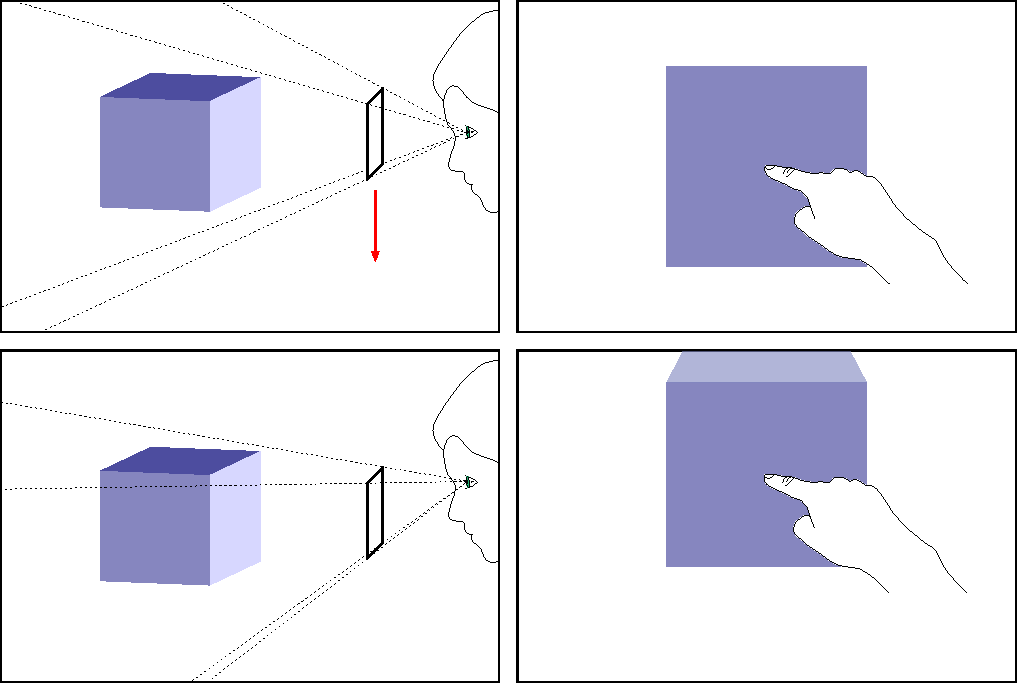
\includegraphics[width=10cm]{img/screen-transformation.pdf}
	\end{center}
	\caption{Translation der virtuellen Bildfläche und die Auswirkung auf die Darstellung.}
	\label{fig:screen-transformation}
\end{figure}

\begin{figure}
	\begin{center}
		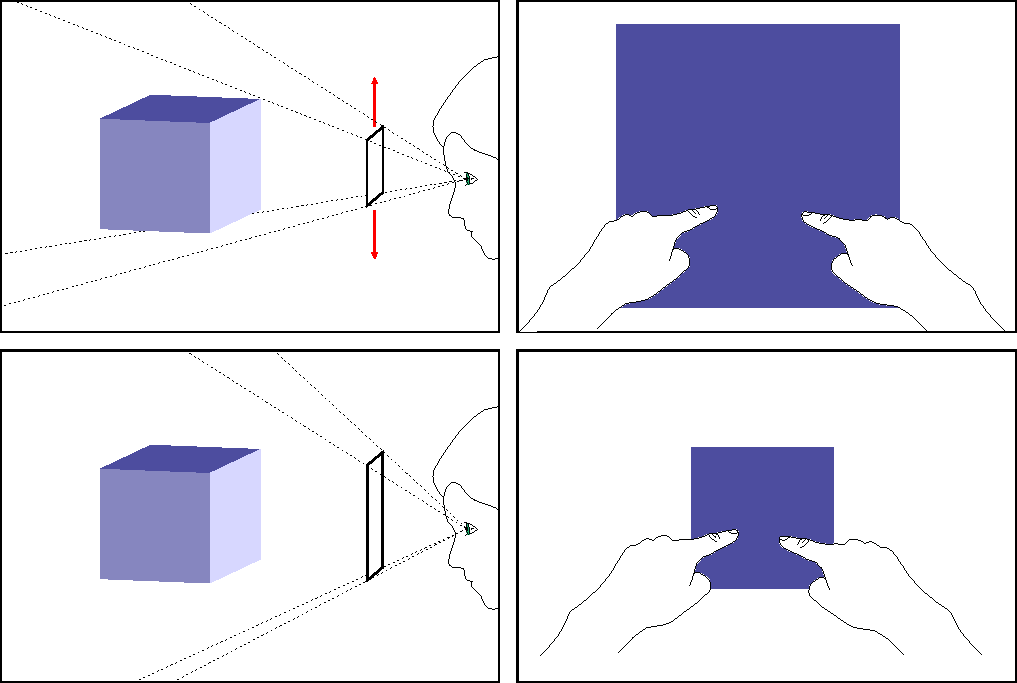
\includegraphics[width=10cm]{img/screen-scale.pdf}
	\end{center}
	\caption{Skalierung der virtuellen Bildfläche und die Auswirkung auf die Darstellung.}
	\label{fig:screen-scale}
\end{figure}

Wird zur Berechnung der Manipulation ein Kontaktpunkt auf dem Bildschirm verfolgt, können mit diesem Ansatz x- und y-Translation der Navigation gesteuert werden. Hierzu ergibt sich die Verschiebung des Viewing-Setups, aus der relativen Bewegung des Kontaktpunkts auf der Projektionsfläche. Die Abbildungen \ref{fig:screen-transformation} und \ref{fig:screen-scale} visualisieren die Auswirkung von Translation und Skalierung des virtuellen Bildschirms.
\\\\
Wir definieren $P_1(t) = (x_1, y_1)$ als die Position des Kontaktpunkts $P_1$ auf der Bildebene, zu einer gegebenen Zeit $t$. $P_1(t‘) = (x_1‘, y_1‘)$ sei die Position von $P_1$ zu einer späteren Zeit $t‘$. Die relative Translation $T_r = (x_r, y_r)$ berechnet sich durch $T_r = P_1(t) – P_1(t‘)$. Um diese Bewegung auszugleichen muss die Navigation um $T = (x_t, y_t) = (-x_r, -y_r)$ verschoben werden.
\\\\
Mit der Verwendung eines zweiten Kontaktpunkts $P_2$ auf dem Bildschirm, wird diese Transformation um die Rotation entlang der Bildschirmnormalen, sowie die symmetrische Skalierung erweitert. Als Referenzpunkt hierfür dient $P_1$.
\\\\
Sei $P_2(t) = (x_2, y_2)$ die Position des Kontaktpunkts $P_2$ auf der Bildebene, zu einer gegebenen Zeit $t$ und $P_2(t‘) = (x_2‘, y_2‘)$ die Position von $P_1$ zu einer späteren Zeit $t‘$, so ergibt sich $V = P_2(t) – P_1(t)$, als Richtungsvektor zwischen den Kontaktpunkten vor der Bewegung. $V‘ = P_2(t‘) – P_1(t‘)$ ist folglich der Richtungsvektor nach der Bewegung. Verändert sich die Distanz der Kontaktpunkte auf der Tischfläche, so muss sich die Distanz der Angriffspunkte auf der Geometrie in gleichem Maße ändern. Die Größenrelation der dargestellten Geometrie kann durch Skalierung der virtuellen Bildebene beeinflusst werden. Der Skalierungsfaktor $S$, bestimmt sich nach diesem Zusammenhang aus dem Verhältnis der Distanzen zwischen den Kontaktpunkten zu den Zeiten $t$ und $t‘$. Folglich gilt $S = |V| / |V‘|$. 
\\\\
Für die Rotation dienen ebenfalls die Vektoren $V$ und $V‘$ zur Berechnung. Als Achse dient die Bildschirmnormale $N$. Diese kann leicht durch $N = ||V|| \times ||V‘||$ bestimmt werden. Der Winkel $\alpha$ für die Transformation ist durch $\alpha = arccos(||V|| * ||V‘||)$ gegeben.


\section{3D Translation}
\label{sec:3d_translation}

Die 3D Translation ist ein von den Erkenntnissen der Balloon Selection nach Benko und Feiner \cite{benko:2007} abgeleiteter Ansatz. Durch \linebreak Berühren  der Tischfläche mit einer Hand wird eine direkte Verbindung mit der darunter liegenden Geometrie hergestellt. Diese zur Tischfläche orthogonale Beziehung soll zu jedem Zeitpunkt der Navigation in diesem Modus gewahrt bleiben. Es leitet sich demnach für die Interaktion mit nur einem Eingabepunkt eine zweidimensionale Translation, nach den in Abschnitt \ref{sec:rst_im_bildraum} beschriebenen Zusammenhängen, ab.
\\\\
Durch die Verfolgung der Bewegung zweier Eingabepositionen, kann eine dreidimensionale Translation abgebildet werden. Hierzu dient einer der verfolgten Kontakte auf dem Tisch als Primäreingabe. Die Bewegung dieser Position bestimmt weiterhin die x- und y-Translation im Bildraum. Der zweite Kontakt wird im Folgenden als Sekundäreingabe bezeichnet. Die Einordnung in Primär- und Sekundäreingabe kann durch Auswertung der Startzeit der jeweiligen Eingabe festgelegt werden. Durch Distanzveränderung der Sekundäreingabe zur Primäreingabe kann die z-Verschiebung gesteuert werden. Zur Berechnung dieser bieten sich zwei verschiedene Verfahren an.
\\\\
Wir definieren $P_1(t) = (x_1, y_1)$ und $P_2(t) = (x_2, y_2)$ als die Positionen der Primäreingabe $P_1$ und der Sekundäreingabe $P_2$ auf der Projektionsfläche, zu einer gegebenen Zeit $t$. $P_1(t‘) = (x_1‘, y_1‘)$ und $P_2(t‘) = (x_2‘, y_2‘)$  seien die Position von $P_1$ und $P_2$ zu einer späteren Zeit $t‘$. Weiterhin werden die Richtungsvektoren $V = P_2(t) – P_1(t)$ und $V‘ = P_2(t‘) – P_1(t‘)$ bestimmt. $z_t$ ist die zu ermittelnde z-Translation.
\\\\
Das erste Verfahren nutzt die Differenz zwischen $|V|$ und $|V‘|$ zur Bestimmung der z-Translation. Bei Verlängerung der Distanz zwischen den Eingabepunkten, soll der Abstand zur darunter liegenden Geometrie in gleichem Maße abnehmen. Bei Verkürzung der Strecke zwischen $P_1$ und $P_2$ wächst die Distanz zur Geometrie um den Betrag der Differenz. Für ein Viewing Setup, mit Blickrichtung entlang der negativen z-Achse, ergibt sich:
\\\\
$z_t = |V| – |V‘|$
\\\\
Der entstehende Effekt lässt sich mit der Anwendung eines Flaschenzugs vergleichen werden. Im zweiten Verfahren wird das Verhältnis zwischen $|V|$ und $|V‘|$ zur Bestimmung der z-Translation genutzt. Verdoppelt sich beispielsweise die Strecke zwischen $P_1$ und $P_2$, so halbiert sich die Distanz zwischen $P_1$ und dem Geometrieauftreffpunkt ($P_g$). $G$ ergibt sich als Richtungsvektor zwischen $P_1$ und $P_g$
\\\\
$z_t = |G| - |G| * \frac{|V|}{|V'|}$
\\\\
Für eine sinnvolle Einbindung beider Ansätze in die Applikation wird die skalierungs-basierte Berechnung von $z_t$ nur angewandt wenn \linebreak $|G| - |G| * \frac{|V|}{|V'|} > |V| – |V‘|$ gilt. 
\\\\
Abbildung \ref{fig:baloon_interaction} visualisiert den Umgang mit diesem Interaktionsmodus. Hierbei wird dem Nutzer eine Visualisierung des manipulierten Auftreffpunktes auf der Geometrie dargestellt, sowie die Verbindungslinie zur darüberliegenden Handposition. Die Gerade zwischen den Eingabepositionen wird ebenfalls visuell referenziert.

\begin{figure}
	\begin{center}
		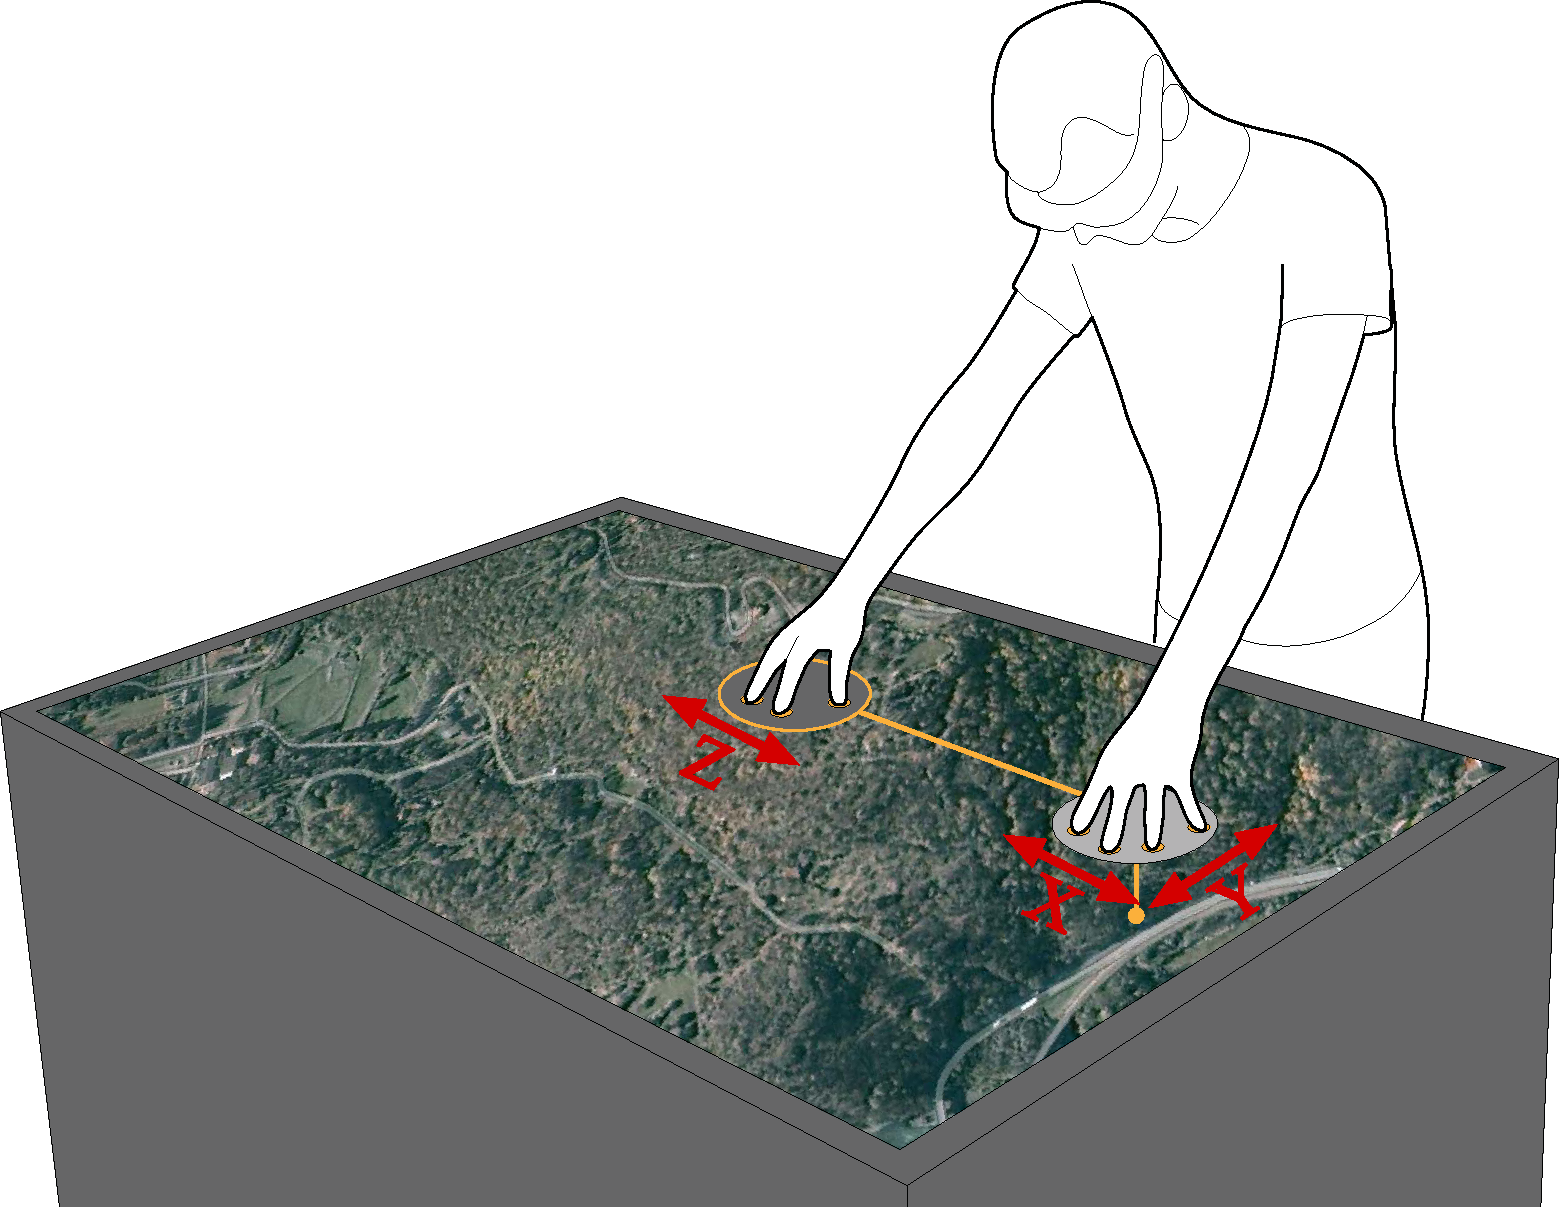
\includegraphics[width=10cm]{img/baloon_interaction.pdf}
	\end{center}
	\caption{Interaktion im 3D Translationsmodus auf Grundlage der Erkenntnisse von Benko und Feiner \cite{benko:2007}. Die roten Pfeile sowie deren Beschriftung sind nicht Teil der Interaktionsvisualisierung}
	\label{fig:baloon_interaction}
\end{figure}

\section{3D Rotation}
\label{sec:3d_rotation}

Ziel dieser Technik ist die Kontrolle aller Freiheitsgrade, welche für die Rotation im dreidimensionalen Raum benötigt werden. Hierzu wurde der in Abschnitt \ref{sec:related_two_axis_valuator} vorgestellte Ansatz von Rousset et al. \cite{rousset:2014} implementiert. 
\\\\
Für die Bestimmung der Manipulation wird die Hand eines Nutzers mit genau zwei aufgesetzten Fingern verfolgt. Initiiert der Nutzer die Geste durch Aufsetzen der Hand, so wird ein direkter Angriffspunkt auf der Geometrie mit orthogonaler Verbindungsgeraden zur Bildschirmfläche berechnet. Bis zur Beendung der Geste durch Anheben der Hand erfolgt eine Rotation um diesen Punkt.
\\\\
Gegeben sind $P_h(t)$ und $P_h(t‘)$ als Positionen des Mittelpunkts der Geraden zwischen den zwei aufgesetzten Fingern zu den Zeiten $t$ und $t‘$. $P_g$ sei der beschriebene Referenzpunkt auf der Geometrie. Zuletzt sind $V_f(t)$ und $V_f(t‘)$, als zeitabhängigen Richtungsvektoren zwischen den Fingern, gegeben. Es werden für die Interaktion zwei Rotationen getrennt voneinander berechnet.

\begin{figure}
	\begin{center}
		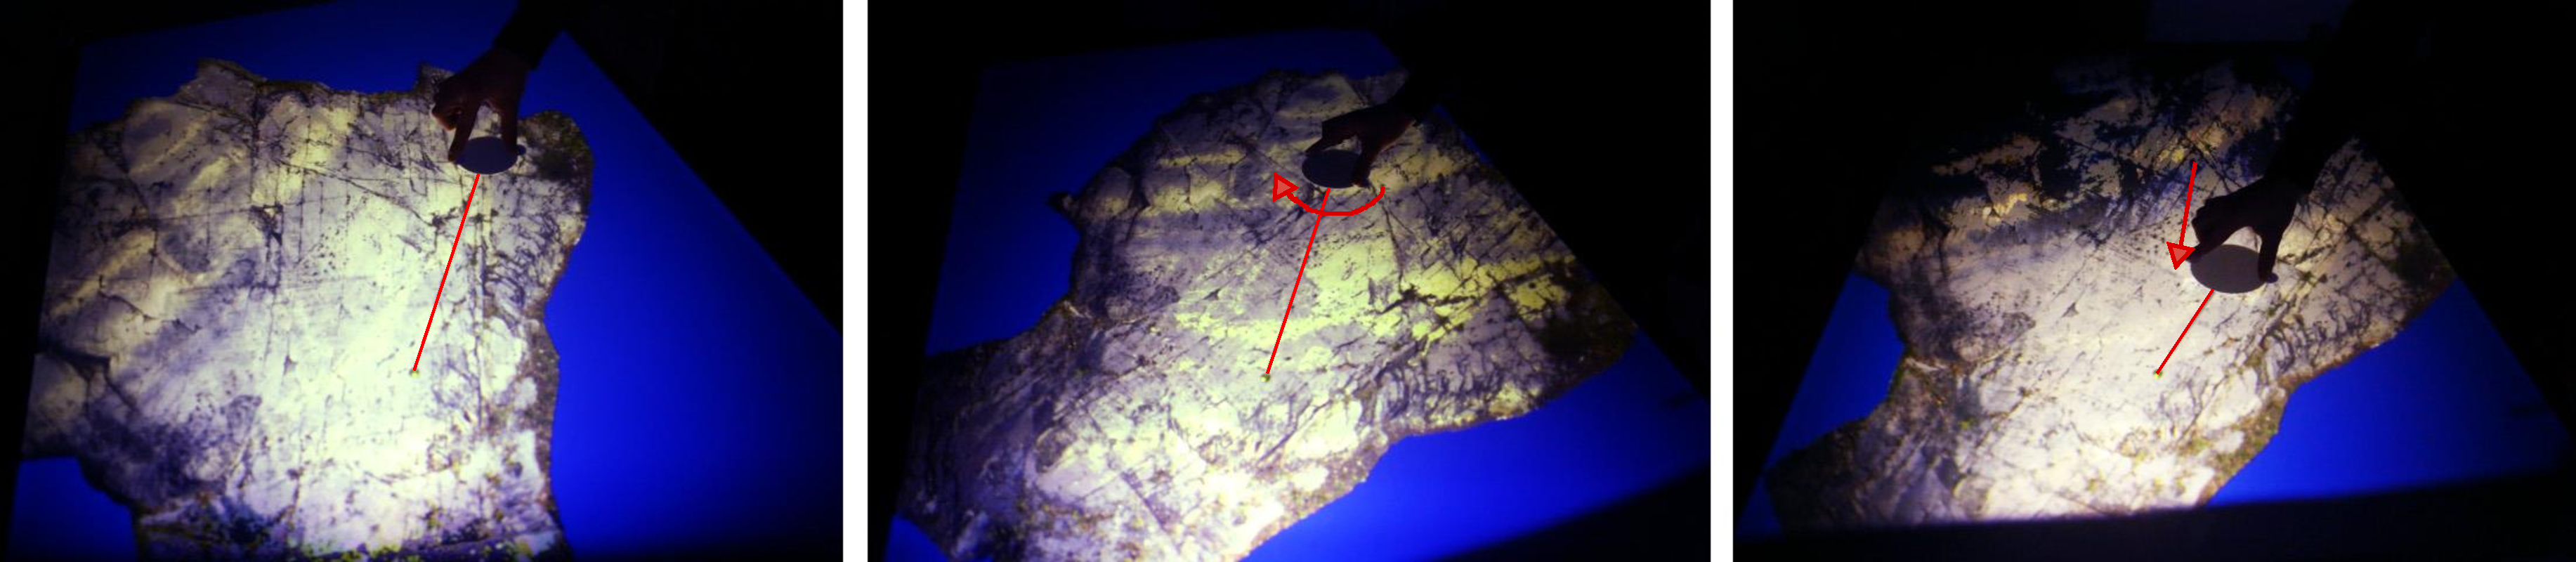
\includegraphics[width=12cm]{img/3d_rotation.pdf}
	\end{center}
	\caption{Interaktion mit dem 3D Rotationsmodus nach Rousset et al. \cite{rousset:2014}.}
	\label{fig:3d_rotation}
\end{figure}

Die Richtungsvektoren $V_{hg}(t)$ und $V_{hg}(t‘)$ ergeben sich aus der Verbindung zwischen $P_h(t)$ mit $P_g$ und $P_h(t‘)$ mit $P_g$. Die Normale auf die von den Vektoren aufgespannte Ebene bildet die Achse der ersten Rotation. Der Winkel leitet sich aus dem Winkel zwischen $V_{hg}(t)$ und $V_{hg}(t‘)$ ab. $V_{hg}(t‘)$ ist außerdem die Achse für eine zweite Rotation, deren Maß durch den Winkel zwischen $V_f(t)$ und $V_f(t‘)$ bestimmt wird. Abbildung \ref{fig:3d_rotation} stellt das Verfahren an einem Beispiel dar.


\section{Vorteile und Limitierungen}
\label{sec:vorteile_und_limitierungen_explizit}

Durch die Verwendung der RTS-Technik (siehe Abschnitt \ref{sec:rst_im_bildraum}) sind eine Vielzahl verschiedener Transformationen im dreidimensionalen Raum gleichzeitig und auch getrennt voneinander zu bedienen. Der anhaltende und direkte Kontakt mit der Geometrie vermittelt dem Nutzer das Gefühl die Szene zu greifen, was zu einer intuitiven Einarbeitung in den Umgang mit dem System führt. Die Technik ist jedoch begrenzt auf dieselben Freiheitsgrade, welche auch im zweidimensionalen Raum verwendet werden. Sie bietet daher nicht die Möglichkeit, die Navigation in jeden durch die drei Dimensionen gegebenen Zustand zu bewegen. Dieser Nachteil spiegelt sich bei den übrigen in diesem Kapitel vorgestellten Techniken noch stärker wieder. Demzufolge ist durch 3D Translation und 3D Rotation jeweils nur eine Form der Transformation steuerbar. Im Kontext ihrer Anwendung zeigen sich beide Techniken ebenfalls als nutzerfreundliche Strategien zur Manipulationen der von ihnen bestimmten Freiheitsgrade.
\\\\
Die Flaschenzugstrategie bei der 3D Translation weist durch ihr direktes Mapping eine hohe Präzision und ein leicht Verständliches Interaktionskonzept auf. Durch die Maße des Tisches und die Reichweite des menschlichen Armes ist der Bewegungsrahmen für die Interaktion eingeschränkt. Ein weit entferntes Objekt in die Nähe der Projektionsebene zu bringen, erfordert somit das wiederholte Anheben und erneute Aufsetzen der Hand. Aus diesem Grund wirkt die Flaschenzugstrategie, bei der Arbeit mit weit entfernten Objekten, ungeeignet. Die Translationsberechnung durch das Verhältnis von Eingabepunkt- und Geometrieabstand kann hingegen effektiv für grobe Interaktionen mit weit entfernten Objekten genutzt werden. Kleine Bewegungen auf der Tischfläche führen zu einer zunehmenden Auswirkung, je weiter das berührte Objekt vom Tisch entfernt liegt. Dementgegen ist die Auswirkung von weitreichenden Bewegungen mit Geometrieelementen in Tischebene gering. Somit entstehen leicht Missverständnisse bei der Nutzung mit bildschirmnaher Geometrie.
\\\\
Die vorgestellte 3D Rotationstechnik kann den Erhalt der Orthogonalität, zwischen dem Geometrie-Eingabe-Vektor und der Bildfläche, nicht gewährleisten. Das hebt die Metapher der direkten Berührung auf, welche sich als nutzerfreundlich erwiesen hat. Wie in Kapitel \ref{chp:wahrnehmungskonflikte_und_loesungsansaetze} beschrieben ist 3D Multi-Touch Interaktion effektiv für Objekte in Null-Parallaxe verwendbar. Bei der 3D Rotation können geringe Eingabeänderungen zu starken Anpassungen des Rotationswinkels führen, wenn die Distanz zwischen Eingabeposition und Rotationsreferenzpunkt gering ist. Befindet sich der Referenzpunkt auf der Tischfläche ist gar keine Berechnung der Rotation mehr möglich. Des Weiteren wird durch den Übergang zwischen Positiv- und Negativ-Parallaxe die Steuerung der Rotation invertiert.


%------------------------------------------------

\chapter{Levelling: Implizite Multi-Touch 3D Navigation}
\label{chp:implizite_navigation}
Kapitel \ref{chp:interaktion_mit_multitoucheingaben} zeigt, dass die gleichzeitige Steuerung aller Freiheitsgrade einer 3D Manipulation durch Multi-Touch Eingaben noch immer eine Herausforderung ist. In Kapitel \ref{chp:explizite_interaktion} werden Lösungsansätze vorgestellt, mit welchen einzelne Freiheitsgrade der Interaktion explizit manipuliert werden können. Ein modulares System zur Koordination dieser Techniken, wäre ein Ansatz mit allen Freiheitsgrade explizit umzugehen. Die Bedienbarkeit eines solchen Systems könnte jedoch leicht komplex werden.
\\\\
Wie Anforderung XX vorgibt soll das System für Nutzer, ungeachtet ihres Vorwissens, leicht handhabbar sein. Um diese Anforderung zu unterstützen beschreibt und evaluiert dieses Kapitel eine im Rahmen dieser Arbeit entstandene Navigationstechnik namens Levelling. Hierzu wird in Abschnitt \ref{sec:definition_levelling} eine Definition zu \emph{impliziter} Navigationstechnik, sowie eine Erklärung zum Interaktionsziel von Levelling, gegeben. Im darauf folgenden Abschnitt \ref{sec:depth_levelling} wird die Funktionsweise von Depth-Levelling beschrieben, während in Abschnitt \ref{sec:rotation_levelling} auf den erweiterten Ansatz Rotation-Levelling eingegangen wird. Abschließend wird in Abschnitt \ref{sec:vorteile_und_limitierungen_implizit} Levelling als Navigationstechnik diskutiert.


\section{Definition und Interaktionsziele}
\label{sec:definition_levelling}

Wir definieren implizite Navigationstechniken als zusätzliche Transformationen zur Erreichung eines Interaktionsziels, welche der Anwendung expliziter Techniken beigefügt werden und nicht getrennt von diesen bedienbar sind. 
\\\\
Bruder et al. \cite{bruder:2013} beschreibt, dass eine effektive Interaktion mit dreidimensionalen Inhalten vor allem möglich ist, wenn Objekte in null Parallaxe liegen. \emph{Levelling} ist ein Ansatz zur impliziten Steuerung der Navigation. Ziel der Technik ist es, nutzerdefinierte Applikationsinhalte auf Tischebene zu bewegen. Es wird dabei sowohl die Distanz der Geometrie zur Bildebene verringert, sowie die Orientierung angepasst. Hierzu legt der Anwender durch berühren des Projektionstisches mit beiden Händen zwei Auftreffpunkte auf der Geometrie fest, welche durch die \emph{Levelling} Technik schrittweise näher an die Bildschirmfläche geführt werden. Da sich beide Punkte auf unterschiedlicher Höhe befinden können, ist außerdem eine Rotation nötig um beide Punkte auf die Bildebene zu führen. \emph{Levelling} ist demzufolge ein zweistufiges Verfahren, dessen einzelne Manipulationsschritte durch die von ihnen hervorgerufene Transformation benannt sind. Abbildung XX. zeigt die Auswirkung von \emph{Levelling} auf eine beispielhafte Visualisierung.
\\\\
Die Punkte auf der Geometrie werden durch einen Schnitttest ausgehend vom jeweiligen Eingabepunkt auf dem Tisch und entlang der Bildschirmnormalen ermittelt. Bei der Schnittberechnung ist wichtig, dass negativ parallaxe Modellbereiche nicht übersehen werden. Folglich muss die z-Koordinate des Startpunkts für den Schnittstrahl\footnote{im Screenspace} auf die Höhe der \emph{Near-Clipping-Plane} angehoben werden. Abbildung XX veranschaulicht diesen Zusammenhang.
\\\\
Wir definieren \emph{Touch-Kontakte} als Strukturen, welche sowohl den Eingabepunkt auf dem Bildschirm, als auch den zugehörigen Geometrieschnittpunkt beinhaltet. Die Orthogonalität der Verbindungsgeraden von Bildschirm- und Geometriepunkt eines \emph{Touch-Kontakts} soll während der Interaktion mit dem Tisch erhalten bleiben. Um dies zu erreichen, muss \emph{Levelling} der Anwendung von RTS im Bildraum (siehe \ref{sec:rst_im_bildraum}) beigefügt werden. Wir nennen diesen Modus Rotation, Translation und Skalierung im Bildraum, erweitert durch \emph{Levelling} (RTS+L).


\section{Depth-Levelling}
\label{sec:depth_levelling}

\emph{Depth-Levelling} wird durch das Eingeben zweier \emph{Touch-Kontakte} initiiert. Nach der Schnittberechnung erfolgt die Einordnung dieser in \emph{Primär-} und \emph{Sekundärkontakt}. Der Geometrieschnittpunkt des \emph{Primärkontakts} liegt näher an der Tischebene oder ist weiter über der dieser als der des \emph{Sekundärkontakts}. Ziel des \emph{Depth-Levellings} ist es, den Geometriereferenzpunkt des \emph{Primärkontakts} durch Translation auf die Projektionsebene zu bringen. Um dies zu erreichen wird das Viewing Setup schrittweise entlang der Bildschirmnormalen verschoben. 
\\\\
Die Schrittweite der Translation wird bei RTS+L durch einen Faktor festgelegt welcher aus der Relation zwischen den \emph{Touch-Kontakte} abgeleitet ist. Ist die Geometrie bereits in relativer Bildschirmnähe, bietet sich die Differenz der Distanz zwischen den Eingabepunkten  seit der letzten Interaktion an. Demnach ist die Levelling-Distanz ($t_L$) gegeben durch:
\\\\
$t_L = | (|V_{S_1S_2}|) - (|V_{S_1S_2}‘|) |$ 
\\\\
,wobei $V_{S_1S_2}$ der Vektor zwischen den Bildschirmpunkten der Touch-Kontakten vor der Eingabe ist und $V_{S_1S_2}‘$ danach. 
\\\\
Für eine größere Translationsdistanz, bei weit von der Bildfläche entfernten Objekten, kann stattdessen das Verhältnis der Länge zwischen $V_{S_1S_2}$ und $V_{S_1S_2}‘$ zur Berechnung von $t_L$ genutzt werden.
\\\\
CALCULATION
\\\\
Abbildung XX zeigt die Auswirkung der verschiedenen Berechnung auf den \emph{Levelling} Vorgang. Sollte die nach einem der genannten Ansätze ermittelte Levelling-Distanz größer oder gleich der Länge des Richtungsvektors zwischen dem Geometrie- und dem Bildschirmpunkt des \emph{Primärkontakts} sein, so wird stattdessen eine Translation um diesen Vektor angewandt. Nach dieser Bewegung befindet sich der Geometriereferenzpunkt des \emph{Primärkontakts} auf Tischebene und das \emph{Depth-Levelling} ist beendet.

\section{Rotation-Levelling}
\label{sec:rotation_levelling}

Das \emph{Rotation-Levelling} schließt sich an die Durchführung des \emph{Depth-Levellings} an. Dieser Vorgang dient der Heranführung des Geometrieschnittpunkts des Sekundärkontakts an die Projektionsebene. Der Modellschnittpunkt des \emph{Primärkontakts} würde durch Translation von der Bildschirmebene entfernt werden. Dies führt zur Aufhebung des durch \emph{Depth-Levelling} erreichten Interaktionsziels. Stattdessen wird eine Rotation um den Bildschirmpunkt des \emph{Primärkontakts} vorgenommen. Desweiteren muss eine Skalierung in Richtung des selbigen Referenzpunkt erfolgen. Mit diesem Schritt soll gewährleistet werden, dass der Richtungsvektor zwischen Geometrie- und Bildschirmpunkt des \emph{Sekundärkontakts} weiterhin senkrecht auf der Bildebene steht.
\\\\
Die Parametrisierung der Rotation bestimmt sich wie folgt.  Sei $G_2$ der Geometrieschnittpunkt des \emph{Sekundärkontakts} und $S_2$ der zugehörige Punkt der Eingabe auf dem Bildschirm, so bestimmt sich $V_{G_2S_2}$ als Richtungsvektor zwischen $G_2$ und $S_2$. Wie beim \emph{Depth-Levelling} (siehe Abschnitt \ref{sec:depth_levelling}) wird im ersten Schritt der Distanzfaktor ($t_L$) für Annäherung an die Bildebene ermittelt. Danach wird ein Punkt $G_2‘$ berechnet, der die Position von $G_2$ nach Verschiebung um $t_L$ entlang $V_{G_2S_2}$ beschreibt. Als nächstes werden zwei Vektoren $V_{S_1G_2}$ und $V_{S_1G_2‘}$ bestimmt. $V_{S_1G_2}$ ist hierbei der Richtungsvektor zwischen dem zugehörigen Bildschirmpunkt des \emph{Primärkontakts} $S_1$ und $G_2$. $V_{S_1G_2‘}$ ist der Richtungsvektor zwischen $S_1$ und $G_2‘$. Der Rotationswinkel ($\alpha_L$) und die Rotationsachse ($R_L = (x, y, z)$) ergeben sich aus:
\\\\
$\alpha_L = arccos(||V_{S_1G_2}|| * || V_{S_1G_2‘}||)$
\\
$R_L = ||V_{S_1G_2}|| \times ||V_{S_1G_2‘}||$ 
\\\\
Wie bereits erwähnt dient eine Skalierung in Richtung des Geometriepunkts des \emph{Primärkontakts} zum Erhalt der Orthogonalität zwischen Geometrie- und Bildschirmpunkt des \emph{Sekundärkontakts}. Der Skalierungsfaktor ($S_L$) ist gegeben durch:
\\\\
$S_L = \frac{|V_{S_1G_2}|}{|V_{S_1G_2‘}|}$
\\\\
Befindet sich der Geometrieschnittpunkt des \emph{Sekundärkontaks} nach Anwendung aller Transformationen auf der Bildebene, so ist das Interaktionsziel erreicht und das \emph{Rotation-Levelling} beendet.


\section{Vorteile und Limitierungen}
\label{sec:vorteile_und_limitierungen_implizit}

Das am Lehrstuhl entwickelte Point Based Rendering  System ermöglicht die Analyse von komplexen 3D Oberflächen-Scans in einem großen Umfang verschiedener Auflösungsstufen. Nach den in Abschnitt \ref{sec:multi_touch_interaktion_mit_3d_szenen} beschriebenen Konzepten, ist die Betrachtung und Interaktion mit dreidimensionalen Modellen vor allem in Bereichen nahe der Projektionseben effektiv möglich. Aus diesem Zusammenhang leitet sich das Interaktionsziel, nutzerdefinierte Inhalte in Bildschirmnähe zu bringen, ab. Durch Anwendung von RTS+L wird der Nutzer ohne Einführung neuer Gesten bei der Erreichung dieses Ziels unterstützt. Hierbei wird die Komplexität der zur Manipulation erforderlichen Transformation vor dem Anwender verborgen.
\\\\
\emph{Levelling} ist als implizite Navigationstechnik nach RTS+L nicht ohne den Einfluss von RTS Bedienbar. Umgekehrt betrachtet können Rotation, Translation und Skalierung bei RTS+L nur getrennt von \emph{Levelling} bedient werden, wenn sich die Geometrieschnittpunkte beider \emph{Touch-Kontakte} auf der Bildebene befinden. 
\\\\
Die am schwersten wiegende Limitierung ist, dass die durch \emph{Levelling} hervorgerufene Manipulation bei RTS+L nicht umkehrbar ist. Demnach schließt RTS+L zwar die z-Translation, sowie 3D Rotation ein, jedoch nur in Richtung der durch die \emph{Touch-Kontakte} definierten Vektoren. Abbildung XX zeigt ein einfaches Beispiel der Folge dieses Problems. Hier wird eine zweidimensionale Fläche windschief zur Tischebene unter dieser positioniert. Nach mehrmaligem Anwenden liegt die Geometrie in der Bildebene. Eine Umkehrung dieses Zustands ist nicht möglich.

%------------------------------------------------

\chapter{Wechsel zwischen Interaktionstechniken}
\label{chp:wechsel_zwischen_interaktionstechniken}
Hier wird das Kapitel Wechsel zwischen Interaktionstechniken beschrieben. Das Kapitel besteht aus den Abschnitten \ref{sec:verhinderung_von_eingabekonflikten} und \ref{sec:interaktionsterritorien}.


\section{Verhinderung von Eingabekonflikten}
\label{sec:verhinderung_von_eingabekonflikten}

Hier steht Inhalt zur Verhinderung von Eingabekonflikten.


\section{Interaktionsterritorien}
\label{sec:interaktionsterritorien}

Hier steht Inhalt zu Interaktionsterritorien.

%------------------------------------------------

\chapter{Virtuelles Freischneiden der Hand während Berühungseingaben}
\label{chp:freischneiden}
Negativ-parallaxe Bildausschnitte können wie in Kapitel \ref{chp:wahrnehmungskonflikte_und_loesungsansaetze} beschrieben Wahrnehmungskonflikte hervorrufen. In diesem  Kapitel wird die im Rahmen dieser Arbeit entstandene \emph{See-Through} Technik basierend auf den Erkenntnissen von Argelaguet et al. \cite{argelaguet:2010} vorgestellt. Die Strategie soll helfen beschriebenen Problemen der Tiefenwahrnehmung entgegenzuwirken.
\\\\
Hierzu definiert Abschnitt \ref{sec:ansatz} den konzeptuellen Ansatz. Abschnitt \ref{sec:implementierung_freischneiden} erläutert die Integration der \emph{See-Through} Technik in die Applikationsstruktur. Zuletzt werden in Abschnitt \ref{sec:vorteile_und_limitierungen_freischneiden} die Vorteile und Limitierungen der Strategie diskutiert.


\section{Ansatz}
\label{sec:ansatz}

\begin{figure}
	\begin{center}
		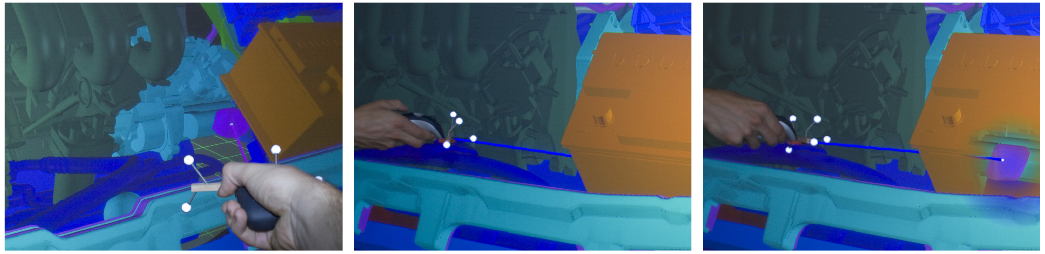
\includegraphics[width=12cm]{img/show_through_related.pdf}
	\end{center}
	\caption{Im linken Bild ist die freie Sicht auf die ausgewählte Geometrie möglich. Diese ist in der mittleren Darstellung verdeckt. In der rechten Abbildung schafft der durch \emph{Show-Through} nach Argelaguet et al. erzeugte Sichtkanal freien Blick auf die verdeckte Geometrie. Diese Abbildung entstammt vollständig einer Veröffentlichung von Argelaguet et al. \cite{argelaguet:2010}} 
	\label{fig:show_through_related}
\end{figure}

Wie in Abbildung \ref{fig:show_through_related} veranschaulicht wird nutzen Argelaguet et al. den von ihnen als \emph{Show-Through} bezeichneten Ansatz zur Freilegung verdeckter virtueller Objekte \cite{argelaguet:2010}. Bei perspektivischem Rendering kann der Blick auf verdeckte Objekte in manchen Betrachtungswinkeln auf der Projektionsfläche sichtbar sein. Die Auswahl dieser Geometrie schafft bei durch \emph{Show-Through} nach Argelaguet et al. einen Sichtkanal auf diese Inhalte für jeden Betrachtungswinkel. Im Kontext dieser Arbeit soll durch Anwendung der Technik die von der Hand des Nutzers durchstoßene Geometrie oberhalb der Projektionsfläche entfernt werden.

\begin{figure}
	\begin{center}
		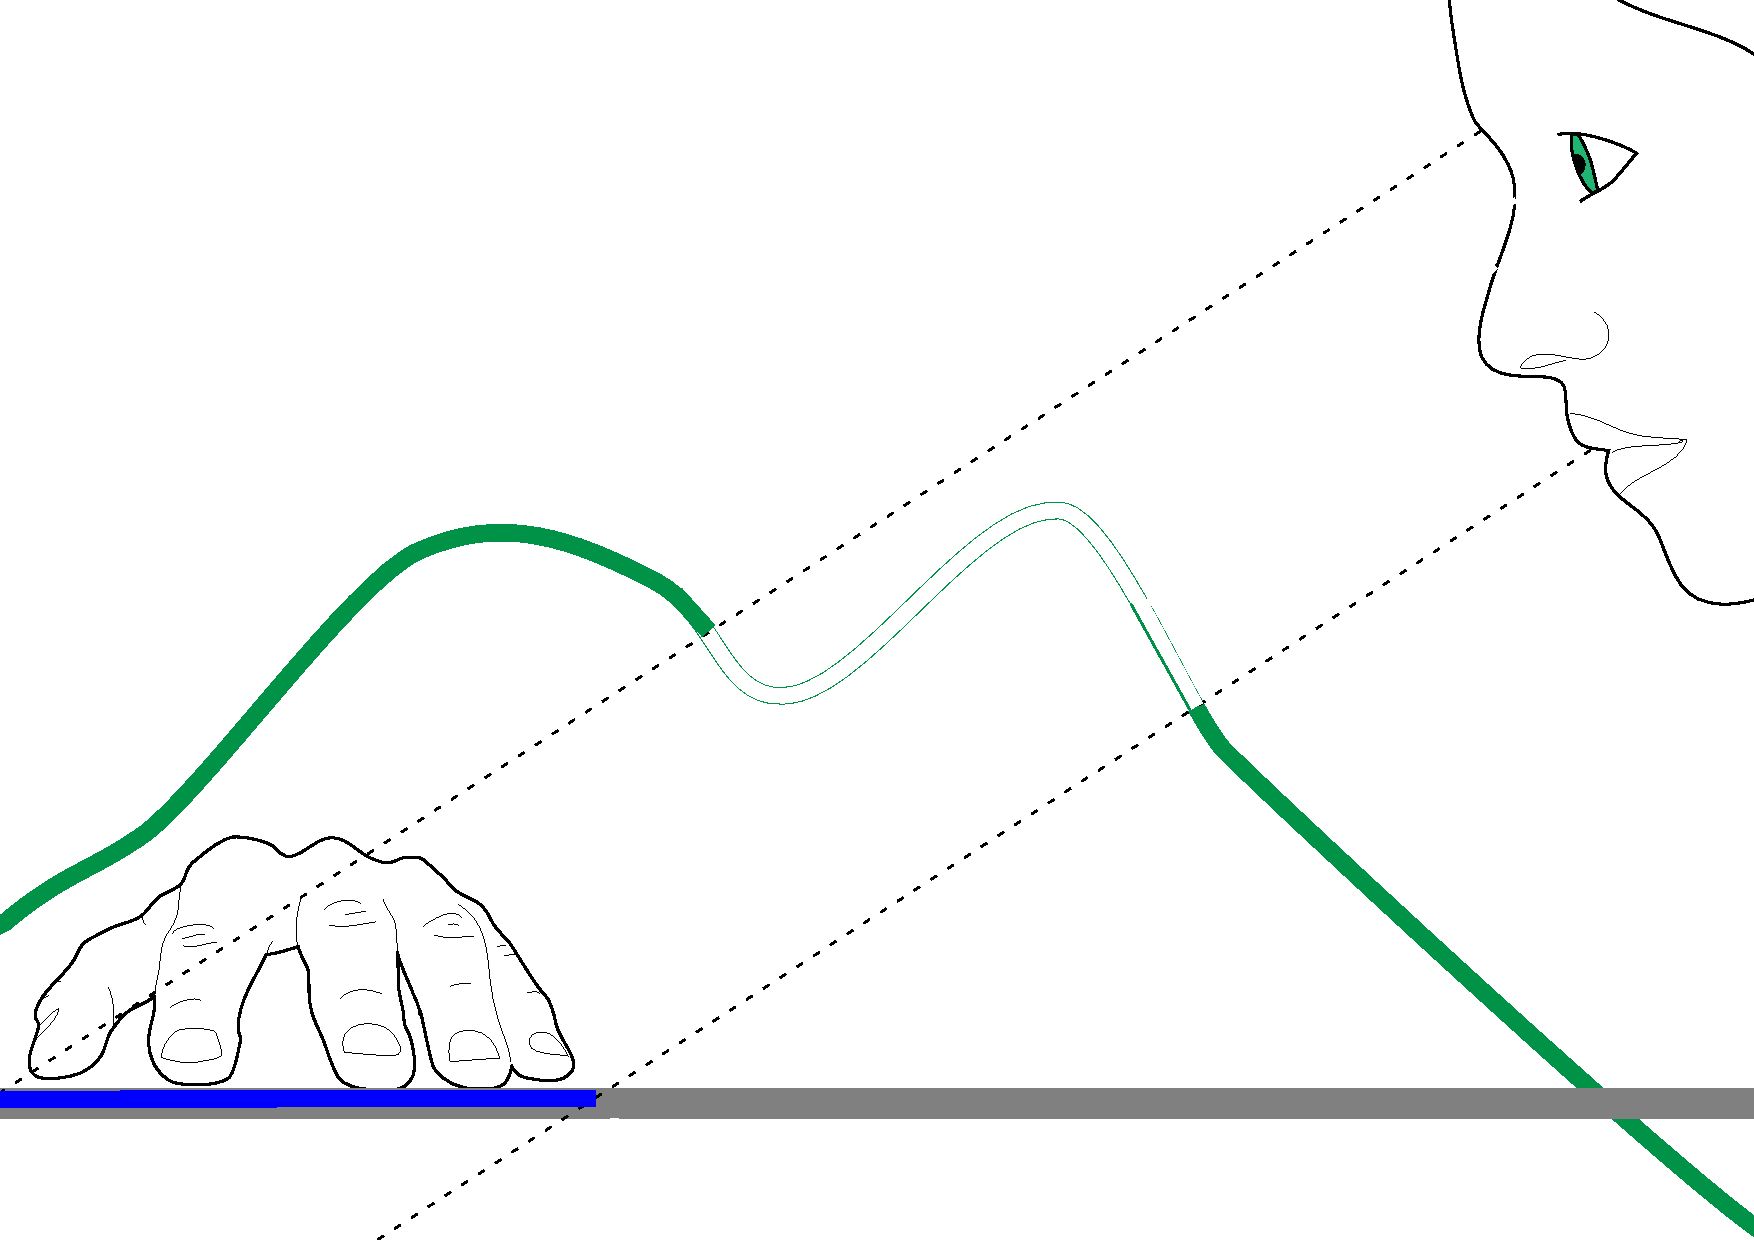
\includegraphics[width=12cm]{img/see_through_1.pdf}
	\end{center}
	\caption{Visualisierung des \emph{See-Through} Konzepts. Die blaue Fläche referenziert das Areal des fingerumschließenden Kreises}
	\label{fig:see_through_1}
\end{figure} 

Wird die Tischoberfläche berührt, so werden negativ parallaxe Modellbereiche zwischen der Eingabeposition und dem Kopf des Nutzers in einem bestimmten Durchmesser ausgeschnitten. Dies erzeugt einen zylinderförmigen Blicktunnel, welcher dem Nutzer freie Sicht bis zu seiner Hand auf der Tischebene bietet. Der Durchmesser des Ausschnittzylinders wird hierbei durch den fingerumschließenden Kreis bestimmt. Abbildung \ref{fig:see_through_1} illustriert die Anwendung der Technik.
\\\\
In einem Mehrbenutzerszenario wird für jeden Nutzer eine eigene Projektion der virtuellen Szene auf dem Bildschirmtisch erstellt. Dies beeinflusst auch die Perspektive auf von Händen verdeckte, negativ parallaxe, Bereiche der Darstellung. Wird für alle um den Tisch versammelten Personen der gleiche Ausschnittzylinder verwendet, kann ausschließlich für einen der Nutzer eine konfliktfreie Wahrnehmung sichergestellt werden.
\\\\
Um Wahrnehmungskonflikte für alle Anwender vermeiden zu können, muss die Orientierung des Ausschnittzylinders nutzerspezifisch angepasst werden. Infolgedessen wird eine eigene Repräsentation des Zylinders für jeden Nutzer bestimmt und auf die jeweilige Projektion angewandt.


\section{Implementierung}
\label{sec:implementierung_freischneiden}

Die Anwendung der \emph{See-Through} Technik kann leicht beim Rendern der Geometriefragmente vorgenommen werden. Hierzu werden alle Eingabepositionen der Hände auf der Tischfläche, sowie der Radius des fingerumschließenden Kreises, in den Fragmentshader der Applikation gegeben. Die Position der Kamera entspricht der Kopfposition des Nutzers und kann somit zur nutzerspezifischen Berechnung der Orientierung des Ausschnittzylinders genutzt werden. Zuletzt werden alle Fragmente, welche innerhalb des Blicktunnels liegen, verworfen.


\section{Vorteile und Limitierungen}
\label{sec:vorteile_und_limitierungen_freischneiden}

Durch die Anwendung der \emph{See-Through} Technik können blickabhängig, von der Hand verdeckte, negativ parallaxe Modellausschnitte bei der Projektion der virtuellen Szene ausgeschlossen werden. Hierdurch bleibt die geometrische Relation zwischen realen und virtuellen Inhalte erhalten. Dies führt zu einer wahrnehmungsunterstützenden Visualisierung, welche maßgeblich zur Benutzbarkeit der Toucheingaben beiträgt.
\\\\
Die \emph{See-Through} Technik beeinflusst lediglich die Darstellung der virtuellen Szene. Eine Manipulation der Geometrie, oder des Blickpunktes, wird nicht vorgenommen. Dadurch kann mit der Szene in jeder geometrischen Lage interagiert werden.
\\\\
Der Zylinder als Ausschnittgeometrie hat sich in der prototypischen Anwendung als gute Approximation des Nutzerarmes erwiesen. Es ist damit möglich den Großteil verdeckter, negativ parallaxer Modellausschnitte, von der Darstellung auszuschließen.
\\\\
Die Ausschnittgeometrie umschließt jedoch ein Volumen, welches nicht exakt die Gliedmaßen des Nutzers repräsentiert. Infolgedessen können Bereiche der Visualisierung beschnitten werden, welche nicht vom Nutzer verdeckt werden und daher noch sichtbar sein sollten. Des Weiteren entspricht die Form und Orientierung der Ausschnittgeometrie nicht der komplexen Form des Arms eines Nutzers. Bei bestimmten Eingaben können somit nicht alle durch Negativparallaxe hervorgerufenen Wahrnehmungskonflikte vermieden werden.
\\\\
Die \emph{See-Through} Technik wird durch das Berühren der Bildschirmoberfläche initiiert. Aus diesem Grund kann das Hineingreifen in Inhalte oberhalb dieser Ebene, ohne Interaktion mit der Tischfläche, nicht verhindert werden.

%------------------------------------------------

\chapter{Diskussion}
\label{chp:diskussion}
In diesem Kapitel soll eine abschließende Diskussion der im Rahmen dieser Arbeit entstandenen Konzepte zur Multi-Touch basierten Interaktion mit stereoskopischen Bildinhalten erfolgen. Hierzu soll die Bewertung dieser Ansätze in Abschnitt \ref{sec:anforderungsevaluierung} anhand der in Kapitel \ref{chp:anforderungsanalyse} definierten Anforderungen bemessen werden. Abschließend werden in Abschnitt \ref{sec:hypothesen} einige Hypothesen definiert die aus Beobachtungen während dem Arbeitsprozess resultieren.


\section{Anforderungsevaluierung}
\label{sec:anforderungsevaluierung}

Der Grundstein für die Entwicklung der Touch Navigation ist durch das \emph{MSER Hand und Finger Tracking} gegeben (siehe Kapitel \ref{chp:mser}). Dieses System bietet eine Reihe von Informationen über die Struktur der Eingabe auf dem Bildschirmtisch. Demnach konnte eine Finger-Hand Zuordnung sinnvoll in der Applikationsstruktur abgebildet werden (siehe Kapitel \ref{chp:applikationsstruktur}). Durch Einführen eines Zusatzkriteriums beim Umgang mit Interaktionstechniken, wurde die maximale Anzahl an für die Manipulation zugelassenen Hände auf zwei begrenzt. Eine Hand-Nutzer Zuordnung wird vom aktuellen System nicht unterstützt. In der Applikation kann die einhändige Eingabe zweier Nutzer somit nicht von der beidhändigen eines Nutzers unterschieden werden. Fehleingaben durch gleichzeitiges Interagieren der Nutzer können folglich nicht vollständig vermieden werden. Nach diesem Zusammenhang wird Anforderung \ref{req:mehrbenutzer} maßgeblich berücksichtigt und unterstützt, jedoch nicht vollständig erreicht.
\\\\
Clipping von Modellbereichen kann Konflikte der Tiefenwahrnehmung durch Stereoparallaxe vermeiden \cite{ardouin:2011}. Das in Kapitel \ref{chp:freischneiden} beschriebene Konzept zur Beschneidung der virtuellen Geometrie, durch einen perspektivabhängigen Ausschnittzylinder nutzt diese Erkenntnis. Abschnitt \ref{sec:vorteile_und_limitierungen_freischneiden} beschreibt, dass die Wahl und Orientierung des Volumens für diesen Prozess nicht der realen Form des menschlichen Arms entspricht. Hierdurch kann nicht vollständig sichergestellt werden, dass der Anwender negativ-parallaxe Modellbereiche nicht berührt. Entstehende Wahrnehmungskonflikte wurden nach Anforderung \ref{req:wahrnehmungskonflikte} abgeschwächt, konnten jedoch nicht gänzlich vermieden werden.
\\\\
Die in die Implementierung der Touch Navigation einbezogenen Techniken ermöglichen dem Nutzer flexiblen Umgang mit virtuellen Inhalten. Hierbei wird die Auswirkung tiefen-anpassender Gesten durch Distanz zwischen Bildschirm und Geometrie skaliert. Angewendete Transformationen sind sowohl im Nahfeld-Bereich als auch auf große Distanz präzise möglich, was das System im Kontext des 3D Pitoti Projekts effektiv nutzbar macht. Anforderung \ref{req:interaktionsziele} wurde nach diesen Kriterien erreicht.
\\\\
Eingebundene Manipulationsformen sind größtenteils am von Hancock et al. vorgestellten Konzept der orthogonalen Verbindung zwischen Geometrie und Bildschirm orientiert \cite{hancock:2007,hancock:2009}. Dies unterstützt das Gefühl Modelle direkt zu Berühren. Nutzer können natürliche Bewegungsabfolgen demnach leicht auf angebotene Navigationsstrategien anwenden. In Kapitel \ref{chp:wechsel_zwischen_interaktionstechniken} wird der Wechsel zwischen den Navigationsmodi vorgestellt. Während die einzelnen Gesten auch für unerfahrene Nutzer leicht steuerbar scheinen, ist das Einprägen der Routine zur Auswahl einer Navigationstechnik nach den in Abschnitt \ref{chp:wechsel_zwischen_interaktionstechniken} Zusammenhängen fraglich. Anforderung \ref{req:intuitiv_benutzbar} wurde im Arbeitsprozess maßgeblich berücksichtigt. Im Hinblick auf zukünftige Entwicklungen sollte eine Studie zur Bewertung der Touch Navigation hinsichtlich dieser Anforderung durchgeführt werden. 
\\\\
Die entwickelten Navigationstechniken ermöglichen die Manipulation aller sechs Freiheitsgrade der Transformation im dreidimensionalen Raum. RST+L bietet die gleichzeitige Kontrolle über x- und y-Translation, z-Rotation und uniforme Skalierung, erweitert durch die implizite Tiefenebnung der \emph{Levelling} Strategie. Mithilfe der 3D Rotation sind die Drehungen um x-, y- und z-Achse getrennt zu bedienen. Der 3D Translations-Modus dient zur expliziten Kontrolle der x-, y- und z-Komponente bei der Bewegungstransformation. Die alleinige Skalierungsanpassung ist nach den in Kapitel \ref{chp:implizite_navigation} beschriebenen Voraussetzungen bei RST+L nur nach Erreichung der Interaktionsziels von \emph{Levelling} möglich. Jedoch kann dies durch menüseitige Filterung der Interaktionsmodi von der Anwendung bei Rotation, Skalierung und Translation im Bildraum ausgeschlossen werden. Somit ist der Skalierungsfaktor auch getrennt von anderen Transformationen konfigurierbar. Anforderung \ref{req:getrennte_bedienung_der_dof} gilt demnach als erfüllt.
\\\\
RST+L gibt dem Anwender die Möglichkeit bekannte Strategien der 2D Touch Interaktion für die Applikationssteuerung einzusetzen. Währenddessen sorgt die Errechnung von Manipulationsparametern bei der \emph{Levelling} Strategie für Ebnung von visuell relevanten Inhalten. Nach Bruder et al. ist die Analyse und Interaktion mit stereoskopischen Geometrien vor allem durch nah an der Bildebene liegende Objekte gegeben. Die Heranführung der vom Nutzer berührten Modelle an die Projektionsfläche ist folglich als Interaktionsziel zu sehen. Nach diesem Zusammenhang ist von der Erfüllung von Anforderung \ref{req:implizite_kontrolle} auszugehen.
\\\\
Zur Visualisierung der Interaktionsprozesse und der taktilen Eingabe wurden verschiedene virtuelle Darstellungen eingeführt. Diese verdeutlichen die Auswirkungen der Interaktion mit der Bildfläche. Sie  verstärken die Verständlichkeit der einzelnen Navigationstechniken und machen fehlerhafte Verarbeitungsergebnisse des MSER Hand und Finger Trackings sichtbar. Somit konnte Anforderung \ref{req:visueller_output} durch das System erreicht werden.


\section{Hypothesen}
\label{sec:hypothesen}

	\begin{hypothese}
	\label{hyp:fehleingaben}
		Fehleingaben der Nutzer können nur durch eine Verbesserung der Eingabeanalyse behoben werden.
	\end{hypothese}

Das MSER Finger und Hand Tracking ist auf die Finger-Hand Zuordnung begrenzt. Dieses Kriterium genügt nicht um Aussagen über die Zugehörigkeit von Eingabepositionen zu einem bestimmten Nutzer zu tätigen. Dadurch können Fehleingaben durch den gleichzeitigen Input mehrerer Anwender von der Applikation nicht vollständig ausgeschlossen werden. Genauer Aufschluss über die Hand-Nutzer Relation ist die Voraussetzung für die Entwicklung von Mechanismen zur Vermeidung beschriebener Mehrbenutzerkonflikte. Die Verbesserung der Eingabeanalyse könnte die Extrahierung dieser Daten ermöglichen.

	\begin{hypothese}
		\label{hyp:konflikte}
		Konflikte der Tiefenwahrnehmung können durch Volume Clipping behoben werden.
	\end{hypothese}
	
Auch wenn die für die See-Through Technik verwendete Ausschnittgeometrie nicht dem menschlichen Arm entspricht, hat sich die Strategie dennoch als große Unterstützung für die kollisionsfreie Tiefenwahrnehmung gezeigt. Eine präzisere Abbildung physischer Gegebenheiten über dem Tisch könnte zu einer geeigneten Konstruktion des Clipping Volumens beitragen.

	\begin{hypothese}
		\label{hyp:unerfahrene}
		Das entwickelte System ist auch für unerfahrene Nutzer leicht zu bedienen.
	\end{hypothese}
	
Abschnitt \ref{sec:diskussion_mser} spricht einige Probleme an, welche durch die Touch Erkennung entstehen. Die Auswirkung dieser beeinflusst drastisch den Umgang mit der Touch Navigation. Aus diesem Grund wurde im Rahmen dieser Arbeit keine Nutzerstudie durchgeführt. Es ist von einer Verzerrung  der Ergebnisse einer potentiellen Studie auszugehen. Testpersonen hätten die offensichtlichen Fehlfunktionen bei der Eingabeauswertung möglicherweise in die Bewertung des Navigationssystems eingebracht. Dieser Zusammenhang stellt die Nützlichkeit der Studienergebnisse zur Evaluierung der Touch Gesten in Frage. Für valide Ergebnisse sollte demzufolge eine Verbesserung der Input Verarbeitung erfolgen.

	\begin{hypothese}
		\label{hyp:levelling}
		Der Umgang mit \emph{Levelling} ist leicht erlernbar und effektiv bei der 3D Multi-Touch Interkation.
	\end{hypothese}
	
Die Berechnung des \emph{Rotation-Levelling} ist gegenüber dem Mapping expliziter Navigationstechniken komplex. Durch den visuellen Effekt der Manipulation wird diese Komplexität jedoch vor dem Nutzer verborgen. Der Zusammenhang die Geometrie durch \emph{Levelling} auf der Bildfläche zu ebnen erscheint schlüssig und leicht zu verinnerlichen. Vor allem im Umgang mit komplexen Oberflächenstrukturen zeigt sich eine automatische Ausrichtungskorrektur anhand nutzerdefinierter Punkte als effektiv.

%------------------------------------------------

\chapter{Fazit}
\label{chp:fazit}
Im Rahmen dieser Arbeit wurde ein System zur Multi-Touch basierten 3D Navigation für einen immersiven Bildschirmtisch implementiert. Hierzu werden verschiedene Techniken zur kollaborativen Exploration virtueller Welten angeboten. Die zur Steuerung der Applikation benötigten Parameter können in spezifischen Gruppen und getrennt voneinander bedient werden. In zukünftigen Arbeiten sollten die eingebundenen Ansätze in einer umfangreichen Nutzerstudie untersucht werden.
\\\\
Entwickelte Modi sind durch die Evaluierung der Bildschirmkontakte vom System unterscheidbar und durch vereinfachte Menüstrukturen vom Anwender zu filter. Die Umsetzung der Erzeugung neuer Menüelemente zur Laufzeit der Applikation konnte im Rahmen der Arbeit lediglich konzeptuell erläutert werden. Es sollte zukünftig eine Implementierung dieser Idee erfolgen.
\\\\
\emph{Levelling} erweitert die expliziten Manipulationsstrategien, um den Nutzer beim Umgang mit den dargebotenen Inhalten zu unterstützen. Unterschiedliche Visualisierungen Referenzieren sowohl die Struktur der Eingabe auf dem Tisch, sowie die Interaktionsvorgänge. Hierbei wäre eine Nutzerstudie zur Effizienzbestimmung des Systems und im Hinblick auf weitere Verbesserungen angebracht. Des Weiteren sollte die \emph{Levelling} Technik einer vergleichenden Betrachtung expliziter Gesten unterzogen werden.  
\\\\
Auftretenden Eingabekonflikten durch einsetzen des Tisches in einem Mehrbenutzerszenario wird durch Analyse der Struktur des Inputs entgegengewirkt. Durch Einbindung der \emph{See-Through} Technik bei Berührung der Projektionsfläche werden negativ-parallaxe Modellbereiche zur Vermeidung von Konflikten der Tiefenwahrnehmung freigeschnitten. Betrachtet man die Bilder die zur Analyse des MSER-Algorithmus genutzt werden, stellt sich die Frage ob weitere Informationen über die Objekte über dem Tisch extrahiert werden können. Aktuell wird lediglich eine zweidimensionale Orientierung des Armes anhand einer die Wurzel-ER umschließenden Ellipse übermittelt (siehe Kapitel \ref{chp:mser}). Es bleibt zu untersuchen ob sich eine dreidimensionale Relation aus den Disparitäten ableiten ließe. Dies würde zur Untersuchung der Hand-Nutzer Zuweisung beitragen. Des Weiteren würde hierdurch eine Basis für die Bestimmung eines präziseren Clipping Volumens bei der \emph{See-Through} Technik geschaffen werden.
\\\\
Die Arbeitsweise der \emph{Touchwerkzeuge} macht die Applikationsstruktur leicht erweiterbar für die Entwicklung zusätzlicher Interaktionsvorgänge welche durch taktile Eingaben gewährleistet werden. Außerdem sind integrierte Navigationstechniken mit einem anderen Input austauschbar. Es wäre demnach interessant zu sehen ob die Techniken auch mit anderen Eingabegeräten sinnvoll in Zusammenhang gebracht werden können.



%------------------------------------------------
%	APPENDIX
%------------------------------------------------

\appendix

%------------------------------------------------

\chapter{Anhang 1}

Im Anhang kann auf Implementierungsaspekte wie Datenbankschemata

oder Programmcode eingegangen werden.


%------------------------------------------------
%	IMAGES APPENDIX
%------------------------------------------------

\listoffigures


%------------------------------------------------
%	TABLES APPENDIX
%------------------------------------------------

\listoftables


%------------------------------------------------
%	REFERENCES
%------------------------------------------------

\bibliographystyle{apalike}    

\bibliography{main_bib}         % verwendet main_bib.bib


%------------------------------------------------
%	END OF DOCUMENT
%------------------------------------------------

\end{document}